
%% This is an example first chapter.  You should put chapter/appendix that you
%% write into a separate file, and add a line \include{yourfilename} to
%% main.tex, where `yourfilename.tex' is the name of the chapter/appendix file.
%% You can process specific files by typing their names in at the 
%% \files=
%% prompt when you run the file main.tex through LaTeX.
\chapter{Introduction}

\section{The Standard Model of Particle Physics}

Physics is the research of relationship between space and time and energy and matter. Physicists enjoy searching for symmetries and consideration laws in nature. They develop elegant mathematical formulations to describe the beauty of the nature and predict or explain the experimental results and observed phenomena. 

There are four known fundamental forces in nature: gravitational force, electromagnetic force, strong force, and weak force. The gravitation force describes the interaction between two massive objects. The electromagnetic force describe the interaction between electrically charged objects. The strong force describes the interaction between nucleons. The weak force describe the radioactive decay of particles. The Standard Model (SM) of Particle Physics is based on theoretical of relativistic quantum field theory with a gauge symmetry of $SU(3) \times SU(2) \times U(1)$ \cite{SMTheory}. It unifies the strong, weak, and electromagnetic into a single theory and describes all particles participating in these interactions. The ingredient of the standard model are lepton, quarks, gauge boson, and Higgs boson shown in Figure~\ref{fig:SMParticle}.

\begin{figure}[hbtp]
\begin{center}
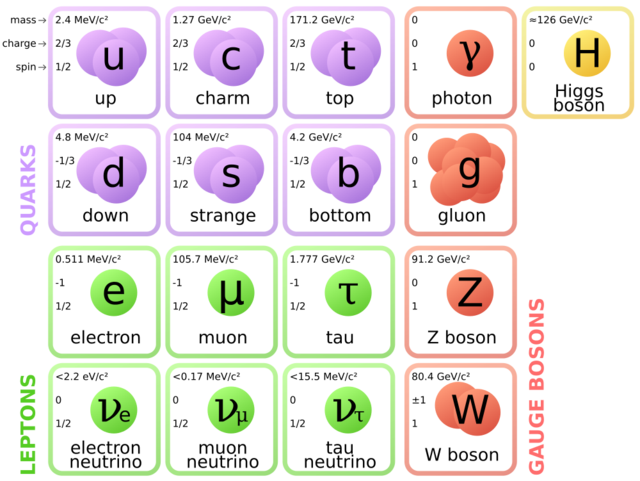
\includegraphics[width=0.50\textwidth]{Figures/Chapter1/SMParticles.png}
\caption{The 17 elementary particles, including leptons, quarks, gauge bosons, and Higgs boson, and their basic properties, such as mass, electric charge, spin, in the Standard Model of Particles Physics are shown above.}
\label{fig:SMParticle}
\end{center}
\end{figure} 


There are 19 parameters in the Standard Model: 6 quark masses, 3 lepton masses, 3 coupling strengths, 4 CKM angles, Higgs mass, vacuum expectation value, and QCD vacuum angle. These parameters are determined from the experiments. Physicists perform calculations based on the Standard Model and predict the cross section of different processes in high energy physics experiments. Since it is proposed in the 1970s, the Standard Model has been tested extensively in countless high-energy physics experiments. Its prediction holds for all of them with very few exceptions. The Standard Model consists of two sectors: the Electroweak theory (EW) and Quantum Chromodynamics (QCD). The Lagrangian of the Standard Model can be written as the sum of EW and QCD: $\mathcal{L_{SM}} = \mathcal{L_{EW}} + \mathcal{L_{QCD}}$ 


\section{Quantum Chromodynamics}

\subsection{QCD Lagrangian}

QCD, a non-abelian gauge theory with $SU(3)$ symmetry, is the theory for the strong interaction between quarks and gluons. The QCD Lagrangian is as follows:


\begin{equation}
\mathcal{L_{QCD}} = \bar \Psi^i i (\slashed{D})_{ij} \Psi^j - m  \bar \Psi^i \Psi_i - \frac{1}{16\pi^2} G^{\mu\nu}_{a}G_{\mu\nu}^{a}
\end{equation}

Where 

\begin{equation}
\slashed{D} = \gamma^\mu \partial_\mu - i g_s \frac{\lambda}{2}  \gamma^\mu A_\mu
\end{equation}

\begin{equation}
G^{\mu\nu}_{a} = \partial^\mu A^\nu_{a} - \partial_{\nu} A^\mu_{a} + g_s f_{abc} A^\mu_b A^\nu_c 
\end{equation}

Here, $\lambda$ are the Gell-Mann Matrices. $f_{abc}$ is the structure of constant of $SU(3)$. $A^\mu$ is the eight gluon field. $g_s$ is the strong coupling constant. The color indices $i$ and $j$ run from 1 to 3, which stands for 3 colors: red, blue, and green. The gluon field indices $a$, $b$, and $c$ run from 1 to 8, standing for the 8 gluon state (Gluon octet as the combination of 3 color and 3 anticolor: $3 \times \bar 3 = 1 \oplus 8$) living in the adjoint representation of $SU(3)$ of color.  



\subsection{Asymptotic Freedom}

The running of the strong coupling constant $\alpha_s = \frac{g_s^2}{4\pi}$ according to the 1-loop calculations in the renomalization theory \cite{QCDRunning} is shown as follows

\begin{equation}
\alpha_{s} (Q^2) = \frac{12\pi}{(11 N_{c} - 2 N_{f}) \ln(\frac{Q^2}{\Lambda_{QCD}^2})}
\end{equation}

We can see that as the energy scale increases, the coupling strength of the strong interaction decreases. This is in contrast to QED where the electromagnetic coupling strength increases as the energy scale increases. In the ultra-violate limit $Q^2 \rightarrow \infty$ and $\alpha_{s} \rightarrow 0$, quarks and gluons behave like free particles. This feature in QCD is call Asymptotic Freedom \cite{QCDAsym}. Meanwhile, in the infrared limit, the strong coupling constant increases. Near the $\Lambda_{QCD} \simeq$100 MeV, the coupling is greater than 1, where the perturbative expansion of QCD breaks down. Experimentally, physicists measure the strong coupling constant at different energy scales from different experiments at different colliders. Figure~\ref{QCDCoupling} \cite{AlphaTheoEx} show the running of strong coupling constant in experiment and comparison with the theoretical calculations 

\begin{figure}[hbtp]
\begin{center}
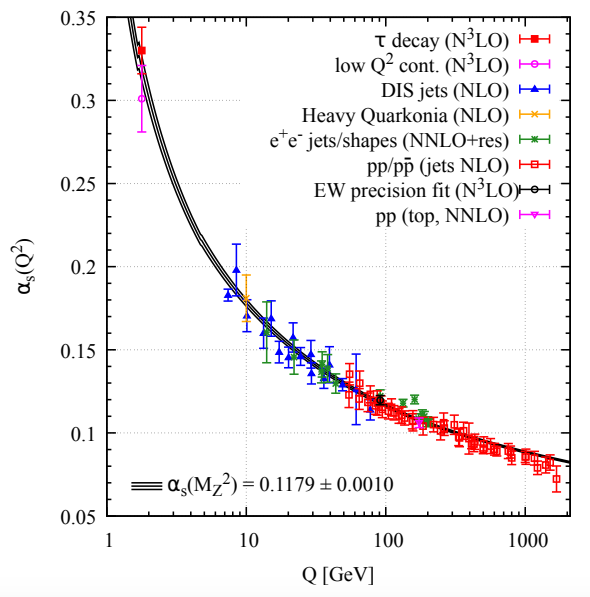
\includegraphics[width=0.50\textwidth]{Figures/Chapter1/QCDCoupling.png}
\caption{The running of the strong coupling constant $\alpha_s$ in different experiments at different energy scale $Q$ and the comparison with QCD calculations are shown above.}
\label{QCDCoupling}
\end{center}
\end{figure} 

An excellent agreement between the theoretical predictions and experimental results of the strong coupling constant is observed in Figure~\ref{QCDCoupling}. 

\subsection{Perturbative QCD}

It is mathematically proven that there is in general no closed form expression for the Standard Model Lagrangian under the Quantum Field Theory framework. Therefore, physicist develop perturbation theory in Quantum Field Theory and apply it to the Standard Model. Physicist obtain asymptotic expansions as power series of the coupling constants and approximately calculate the expectation values of the observables to prediction experimental results.

For QCD, in high energy and hard scattering processes, since the coupling constant is much less than 1, perturbation theory is applicable to QCD. Feynman rules and diagrams are applicable in the matrix element to evaluate the cross section of hard parton-parton scattering. Perturbative QCD (pQCD) calculations have been tested various experiments such as electron positron annihilation, deep inelastic electron proton scattering, and high energy proton-proton collisions.

\subsection{Non-perturbative QCD}

At low energy and soft scattering processes, the coupling constant is greater than 1, perturbation theory of QCD breaks down. Many low-energy QCD processes such as hadronization and hadron-hadron interactions are non-perturbative. Historically, physicists developed Lattice gauge theory such as Lattice QCD to calculate the mass \cite{LQCDProtonMass} of the proton and effective theory such as Chiral Perturbation Theory to study pion-nucleon scattering \cite{ChiPT}. Non-perturbative QCD have achieved many successes. Currently, many novel developments applying non-perturbative QCD to understand nuclear structure and nucleon spin structure are being carried by physicists.

\subsection{QCD Factorization Theorem}

The QCD factorization theorem states that in events involving both hard and soft QCD processes, hard and soft process are mathematically factorized in the cross section computation as follows \cite{QCDFactorization}: 

\begin{equation}
\sigma_X = \Sigma \int dx_1 dx_2 f_i(x_1,\mu_F^2) f_j(x_j,\mu_F^2) \times \hat \sigma_{ij\rightarrow X} (p_1,p_2,\mu_R^2,\mu_F^2)  
\end{equation}

\begin{figure}[hbtp]
\begin{center}
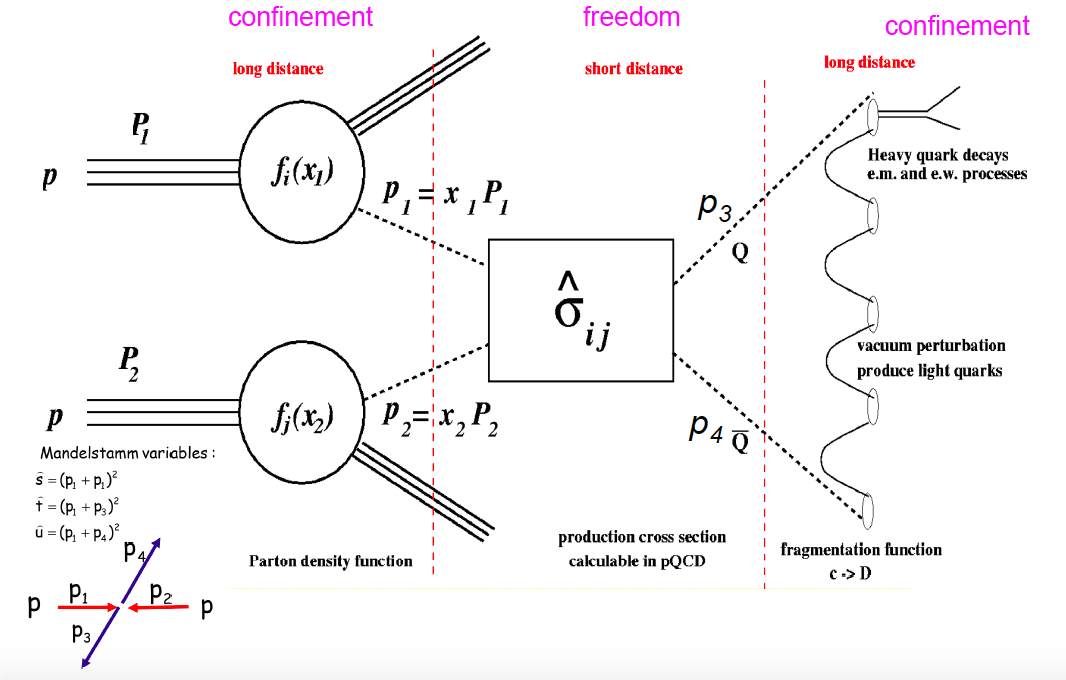
\includegraphics[width=0.75\textwidth]{Figures/Chapter1/QCDFactorizationTheorem.png}
\caption{The QCD factorization theorem applied to a pp collision event involving in soft and hard processes are shown above.}
\label{QCDFacTheo}
\end{center}
\end{figure} 

The hard processes are encoded in the factor of partonic cross sections while the soft processes are measured in experiments. Physicists developed parton distribution function to describe initial kinematic of partons inside hadrons and fragmentation function to describe the parton hadronization process. Both parton distribution function and fragmentation function are measured in experiments.


Physicists apply QCD factorization theorem to perform pQCD calculation of hard scattering processes and use the measurement from the  to understand the hadron spectroscopy in electron-positron, electron-proton, and proton-proton collisions.

\subsection{Color Confinement}

Another feature of QCD as a non-abelian gauge theory is color confinement. The strong force carrier gluon itself is also color charged. Color charged partons, namely quarks and gluons, are never detected in isolation. In experiments, only color neutral hadrons are detected. Currently, the analytic explanation of color confinement is still not yet rigorously proven. The theoretical explanation of color confinement in QCD remains one of the unsolved problem in physics. 

\subsection{Hadronization}

The formation process hadrons from partons is called haronization. Because in experiments we only measure final state hadrons, in order to study the interactions and dynamics of quarks and gluons during partonic stage from hadron spectra, we also need to understand hadronization mechanisms. However, hadronization is in general non-perturbative and cannot yet be described by first principle QCD calculations. Therefore, physics make phenomenological models such as the Statistical Hadronization Model \cite{SHM}, Lund String Model \cite{LSM}, Quark Coalescence Model \cite{QCM} to study hadronization. Figure  \ref{HadMech} shows the schematics of hadronization of a beauty quark via fragmentation and coalescence process.

\begin{figure}[hbtp]
\begin{center}
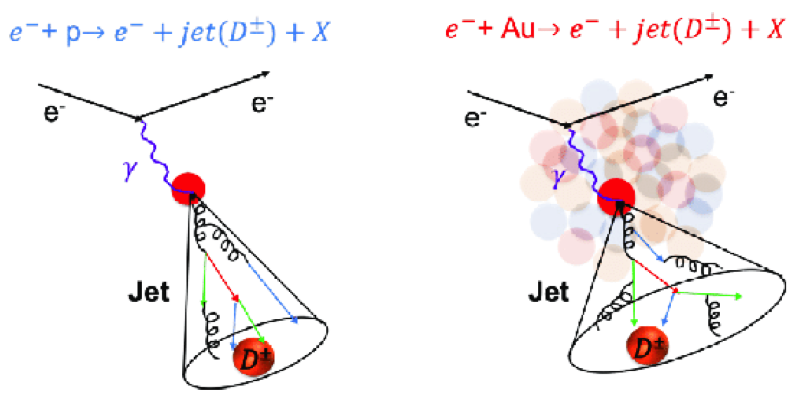
\includegraphics[width=0.48\textwidth]{Figures/Chapter1/FragCartoon.png}
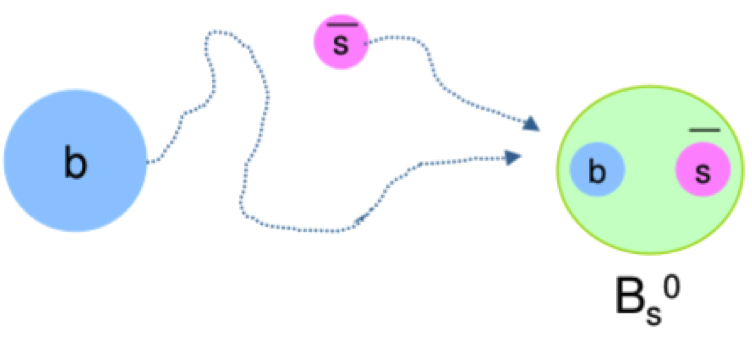
\includegraphics[width=0.48\textwidth]{Figures/Chapter1/CoalCartoon.png}
\caption{The fragmentation process of charms quarks hadronize into $D^\pm$ (left) and the coalescence process of beauty quark with a strange quark nearby to form a $B^0_s$ are shown above.}
\label{HadMech}
\end{center}
\end{figure} 

\section{QCD In Extreme Conditions}

Historically, many efforts to understand QCD in extreme conditions have been made \cite{QCDExtreme}. There are mainly two directions: temperature and parton density. Figure~\ref{QCDConds} shows the different studies of QCD in different conditions \cite{QCDDiffConds}:


\begin{figure}[hbtp]
\begin{center}
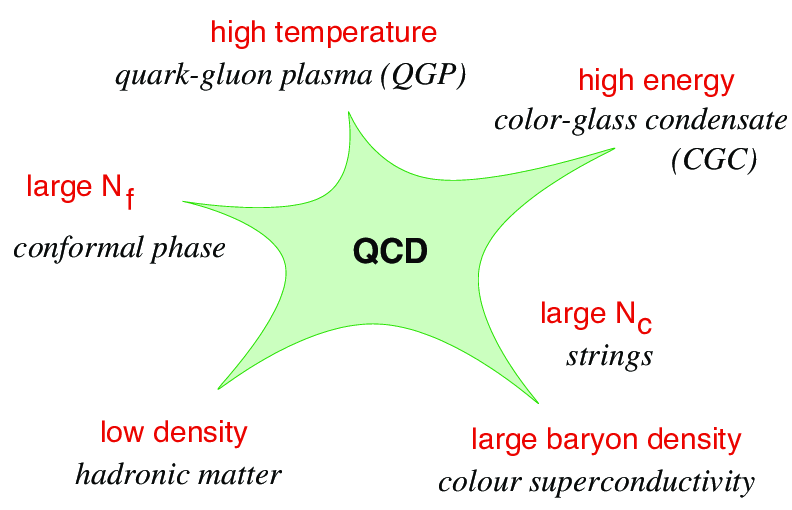
\includegraphics[width=0.70\textwidth]{Figures/Chapter1/ManyBodyQCD.png}
\caption{Many-body dynamics of QCD in different physics limits is shown above.}
\label{QCDConds}
\end{center}
\end{figure} 

\subsection{QCD at Finite Temperature}

In QCD, under extremely high energy density, the degree of freedom of the system increases via particle production. Many-body dynamics become relevant. In the limit of large number of quarks and gluons, after a sufficiently long period of time, the system reach thermal equilibrium via the strong interaction \cite{MLBThermal,ADSCFTThermal,QCDThermal}. Therefore, a description based on thermodynamics can be formulated to study such systems \cite{QCDThemDyn}. We call this thermalized and strongly interacting many-body system of quarks and gluons to be QCD matter.

Therefore, an additional variable temperature ($\mathbf{T}$) can be introduced to study such QCD systems. There are some interesting QCD phenomenologies involving temperature as listed in the following subsections.

%\vspace{1.0cm}

\subsection{Melting of QCD Vacuum}

The QCD vacuum is filled with various condensates of quarks-antiquark pair and gluon fields \cite{QCDVacuum}. In the QCD vacuum, the three flavor of light quarks: $u$, $d$, $s$ form a flavor symmetry group of $SU(3)_f$. However, for quark-quark pair, the $SU(3)_f \times SU(3)_f$ chiral symmetry is spontaneously broken. For example, in the vacuum, a quark-antiquark pair field has a non-vanishing expectation value of $\bra{0} \bar \psi (x)  \psi(x) \ket{0} \simeq$ (250 MeV)$^3$ \cite{}. Therefore, in the physical QCD vacuum, all color field are confined in hadrons. In 1974 T.D. Lee formulated the idea that the non-perturbative vacuum condensates could be ``melted down ... by distributing high energy or high nucleon density over a relatively large volume'' \cite{StockR,QCDVacMelt}. As the energy density in space increases, the color field start to permeate all space. This is effective melting the QCD Vacuum as the temperature of the system increases. Therefore, the temperature of the system will affect the QCD vacuum structure. 

%\vspace{1.0cm}

\subsection{Chiral Symmetry Restoration}

At a finite critical temperature $T_c > 0$, the quark-antiquark pair field will have a vanishing expectation value. In this scenario, massive quarks behave as if massless \cite{ChiralTemperature}. Thus, the chiral symmetry of quarks is restored \cite{ChiralRestore}. Therefore, under a strong magnetic field, due to the restored chiral symmetry, the quarks generate anomalous chiral current $j^{\mu}_{5}$ described by $U(1)_A$ chiral anomaly, calculated by the famous ``Triangle Feynman diagram'' in Figure~\ref{ChiralFeynman} shown below:



\begin{figure}[hbtp]
\begin{center}
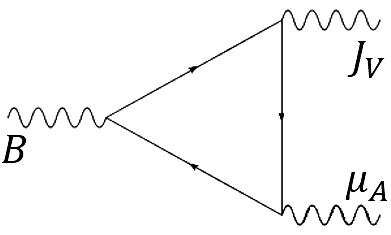
\includegraphics[width=0.45\textwidth]{Figures/Chapter1/ChiralTriangle.png}
\caption{The Feynman diagram of a triangular quark loop under external magnetic field $B$ describe the generation of chiral magnetic current via chiral anomaly is shown above.}
\label{ChiralFeynman}
\end{center}
\end{figure} 


The anomalous chiral current $j^{\mu 5}$ is given by \cite{ChiralPaper}

\begin{equation}
\partial_\mu j^{\mu}_{5} =  - \frac{N_{f}g^2}{16 \pi^2} G^{\mu\nu}_a \widetilde{G^a_{\mu\nu}}
\end{equation}

Here $G^{\mu\nu}_a$ is defined as

\begin{equation}
\widetilde{G^a_{\mu\nu}} = \frac{1}{2} \epsilon_{\mu\nu\lambda\sigma}G^{\lambda\sigma a}
\end{equation}


According to the continuity equation of chiral current

\begin{equation}
\frac{\partial \rho_5}{\partial t} + \nabla \vec{j_5} = 0 
\end{equation}

By definition, the chiral current $\rho_5$ is the difference of the right-handed charge $\rho_L$ and left-handed charge $\rho_R$.


In terms of number of particles $N_5 = \frac{Q_5}{e} = \int  {\rho_5}{e} d^3x$, integrating both sides by the spatial volume and divide by the volume, we have



\begin{equation}
\frac{d N_5}{dt} =  \int d^3x \nabla \vec{j_5} = \int  - \frac{N_{f}g^2}{16e \pi^2} G^{\mu\nu}_a \widetilde{G^a_{\mu\nu}} d^3x 
\end{equation}


The chiral chemical potential $\mu_5$ is proportional to the number of particle $N_5$: $j_5 \propto N_5$ This non-vanishing anomalous chiral current implies non-zero chiral magnetic dipole moment density $\mu_5 \ne 0$. Finally, under an external magnetic field, the induced electric current $j^\mu_V$ is given by  


\begin{equation}
\vec J_V = \frac{N_c e}{2\pi^2} \mu_A \vec B \ne 0
\end{equation}

In experiments, we should expect to see the separation of left-handed and right-handed quarks $Q_V$ due to this electric current $\vec J_V$ where charge imbalance between the positive and negative direction along the magnetic field \cite{CMESignature} as $\Delta Q = \int_0^\tau \vec J_V \cdot \vec A dt \ne 0$. We call this chirality imbalance effect due to the restored chiral symmetry of quarks at finite temperature as \textbf{Chiral Magnetic Effect} \cite{RestoreCME}. Figure~\ref{ChiralScheme} illustrates the schematics of Chiral Magnetic Effect in Heavy-Ion Collisions \cite{CMEFigPaper}

\begin{figure}[hbtp]
\begin{center}
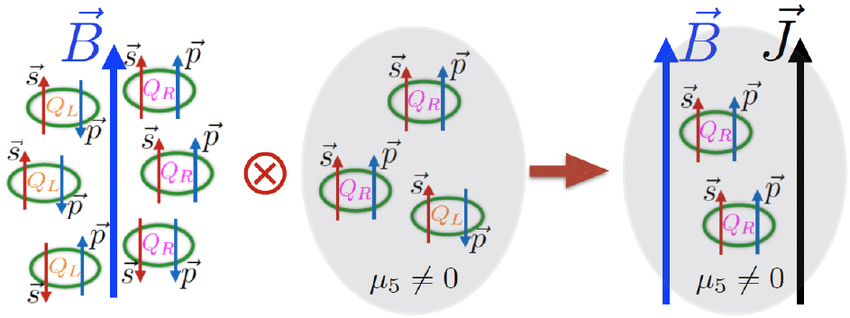
\includegraphics[width=0.70\textwidth]{Figures/Chapter1/ChiralScheme.png}
\caption{The schematics of charge separation due chirality imbalance of quarks under a strong magnetic field in heavy-ion collisions, know as Chiral Magnetic Effect, is shown above.}
\label{ChiralScheme}
\end{center}
\end{figure} 


Currently, physicists are actively looking for evidences of Chiral Magnetic Effect in experiments but have not yet reported any conclusive results so far \cite{CMEExpResult}. 

%\vspace{1.0cm}

\subsection{Temperature Dependence of QCD Static Potential}. 

If we consider two color charged quarks in the limit of infinite mass and are essentially at rest in the lab frame, we can define a QCD static potential between these two quarks due to the strong interaction. In vacuum, such a potential is called ``Cornell Potential'' \cite{Cornell}. The potential as a function of the distance between two quarks is shown as follows:

\begin{equation}
V(r) = -\frac{\alpha_{eff}}{r} + \sigma r
\end{equation}

Here, $\alpha_{eff}$ is the effective strong coupling coupling between the two quarks and $\sigma \simeq 0.184$ GeV/c is the string coupling constant \cite{CornellEquation}. 

Now if we consider at finite temperature $T$ with a thermalized system  between the two quarks, the QCD static potential becomes: 

\begin{equation}
V(r) = -\frac{\alpha_{eff}}{r} e^{-m_D r} + \frac{\sigma}{m_D} (1 - e^{-m_D r})
\end{equation}

Here, $m_D \sim g_s T$ is the Debye mass due to Debye color screening effect \cite{CSEff}, which essentially modifies the gluon propagator by inserting a finite mass term: $-i \frac{g^{\mu\nu}}{q^2} \rightarrow -i \frac{g^{\mu\nu}}{q^2 - m_D^2}$. In fact, Equation (2) reduces to the Cornell potential when T = 0. The QCD static potential is shown below in Figure~\ref{QCDPotential} \cite{TDepCornell}


\begin{figure}[hbtp]
\begin{center}
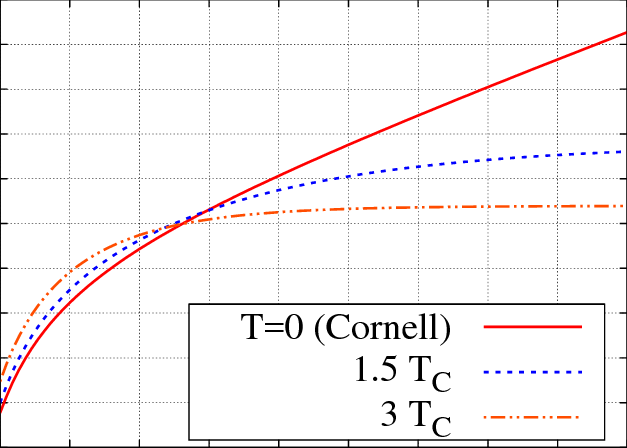
\includegraphics[width=0.45\textwidth]{Figures/Chapter1/QCDPotential.png}
\caption{The QCD potential $V(r)$ from at zero and at finite temperatures as a function of distance $r$ is shown above. Here, the critical temperature $T_c $ = 192 MeV. We can see that the QCD saturates at a finite value at finite temperature. }
\label{QCDPotential}
\end{center}
\end{figure} 

Many interesting physics implications can be derived from QCD at finite temperature.


\subsection{Hadron Mass Spectrum and Hagedorn Temperature}

In 1965, Hagedorn proposed a statistical thermodynamically bootstrap model, giving the temperature dependence of hadron spectra \cite{Hagedorn}. According to the principle of asymptotic bootstrap, in the limit of high mass resonance $m \rightarrow \infty$ the mass spectrum of hadrons $\rho(m)$ grows exponentially 

\begin{equation}
\rho (m) \propto m^{-\frac{5}{2}} e^{\frac{m}{T_0}}
\end{equation}

Here, $\rho(m)$ dm stands for the number of excited hadron with mass between $m$ and $m+dm$. $T_0 \simeq 158$ MeV is the temperature parameter extract from experiments. As $T \rightarrow T_0^-$, $\rho(m) \rightarrow \infty$. The mass spectrum of hadrons diverges. Therefore, it stands for the highest possible temperature achievable for the strong interaction between hadrons. Hence, $T_0$ is also called the ``Hagedorn Temperature''. For $ T > T_0$, the description of color-neutral hadrons mass spectrum will break down, indicating a new type of matter with deconfined degree of freedom in the interaction \cite{HagedornDeconfine}.

\subsection{Color Deconfinement}

As mentioned in the sections above, we see that, at finite temperature, the QCD static potential is screened and color degree of freedom become relevant in the system. As the temperature of the system increase, the quarks and gluon inside color-neutral hadrons will have more available space to move around and start to deconfine \cite{DeconfineTemp}. At some critical temperature $T_c$, quarks and gluons will form a new type color deconfined QCD matter, which is called Quark-Gluon Plasma (QGP). The typical temperature of QGP is in the order of a few hundred MeV or about $10^{12}$ K, which is about hundreds of thousands times hotter than the core of the Sun.

\subsection{QCD at High Parton Density}

In the other direction, while keeping zero temperature, by increasing density of the color fields of the system, another form of QCD matter will also emerge \cite{CondensedQCD}. Due to confinement, a single quark or gluon cannot exit in vacuum. Therefore, the simplest form of QCD system will be a meson, which consist of one quark and one antiquark. The next more complex system will be baryon, for instances, nucleons, which consistent of three quarks. We can then use nucleons to form atomic nuclei and even neutron stars. As the number of nucleons in the system increases, the nucleon density also increases, which increase the color field density. Below, we will discuss the consequence of increasing color field density by increasing the color field lines and decreasing the volume of the system. In general, we can study QCD at High Parton Density by probing small$-x$ physics \cite{SmallX}  


\subsection{Color Glass Condensate}

One way to increase the color field density is by decreasing its volume. The radius of a hadron will shrink due to the Lorentz contraction effect as it moves with respect to the spectator. However, since the number of color charges inside the does not change, the color field density will increase. According to the parton distribution function (pdf), at small $x$, the gluon pdf will dominate. Hence, at very high energy, which is equivalent to small $x$, the hadrons will turn into ``gluon walls'' \cite{GluonWalls} and form a dense color field of matter \cite{DenseColorField} named Color Glass Condensate (CGC) is formed \cite{CGCPaper}. %Figure \ref{CGC} below shows the a simplified version of schematics to visualize CGC of a hadron

\subsection{Gluon Saturation}

However, it is believe that color density of a hadron will not increase indefinitely due to gluon splitting process: $g \rightarrow gg$. At very small $x$, recombination of gluons: $gg \rightarrow g$ also occurs. These two processes compete and eventually balance. They result in a equilibrium color density or, equivalently, a saturation scale $Q_s^2$ \cite{GSIntro}. We call this phenomenon as gluon saturation. Gluon saturation can be described by QCD evolution equations \cite{DGLAP1,DGLAP2,DGLAP3,BFKL,JIMWLKBK}. Figure \ref{GSScalePlot} below shows schematically the different state of a hadron in the double-log scale plot of energy landscape $\ln x$ and the virtuality $\ln Q^2$ \cite{GluonSatuPlot}

\begin{figure}[hbtp]
\begin{center}
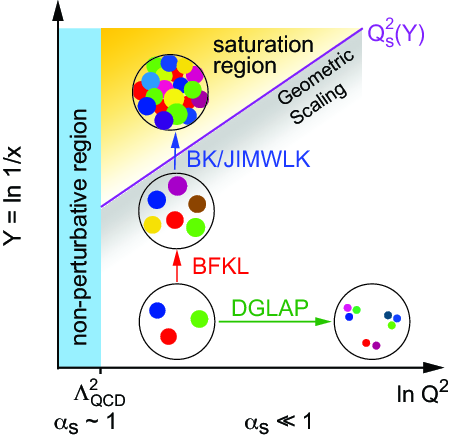
\includegraphics[width=0.45\textwidth]{Figures/Chapter1/GSScalePlot.png}
\caption{The double-log scale of energy landscape $\ln x$ and the virtuality $\ln Q^2$ diagram picturing the different regimes of the hadron wave function, the saturation line separates the dilute (DGLAP) regime from the dense (saturation) regime is shown above.}
\label{GSScalePlot}
\end{center}
\end{figure} 

At the EIC, experiments will also be capable of precisely investigating gluon saturation effects through dihadron correlations analysis \cite{EICGSDIH}.


\subsection{Nuclear Shadowing}

At high energy, or equivalently, small $x$, according to the QCD evolution equation, the gluons inside the nucleon of the nuclei will ``create shadows" on each other \cite{IntroShadow}, The high density effects results in the modification of the nuclear structure function and the gluon nucleon parton distribution \cite{DenseQCD}. Therefore, in high energy hadron-nucleus collision, we expect to see the decrease of cross section per participant nucleons at small-$x$ region compared other $x$ region \cite{ExShadow}. We call this effect as ``nuclear shadowing (of gluons)'' \cite{NuclearShadowing}. 



\section{QCD Matter}

\subsection{QCD Phase Diagram}

Similar to form everyday matters such as metal, water, wood, glass, and plastic, which are formed by electromagnetic interaction and could all be described macroscopically by equations of states that are parameterized by thermodynamic variables. Figure~\ref{QEDPhaseDiagram} shows the phase diagram of water ($\mathrm{H_2O}$) at different temperature and pressure:

\begin{figure}[hbtp]
\begin{center}
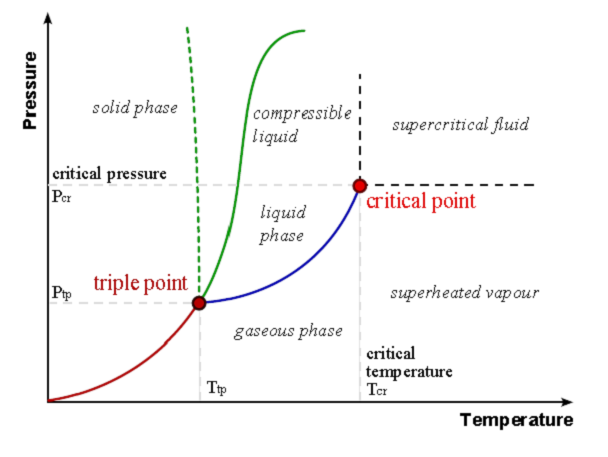
\includegraphics[width=0.45\textwidth]{Figures/Chapter1/WaterPhaseDiagram.png}
\caption{The P-T diagram of water in gas, liquid, solid phases is shown above.}
\label{QEDPhaseDiagram}
\end{center}
\end{figure} 


Similarly, QCD matter is the matter formed by numerous quarks and gluons via the strong interaction and can also be describe by equations of states. Like our everyday matter which has gas, liquid, and solid phases at different pressure and temperature, QCD matter also has different phases at different temperature and baryon chemical potential. and can be describe by QCD phase diagrams. Figure~\ref{QCDPhaseDiagram} shows the QCD phase diagram at different temperature and baryon chemical potential:

\begin{figure}[hbtp]
\begin{center}
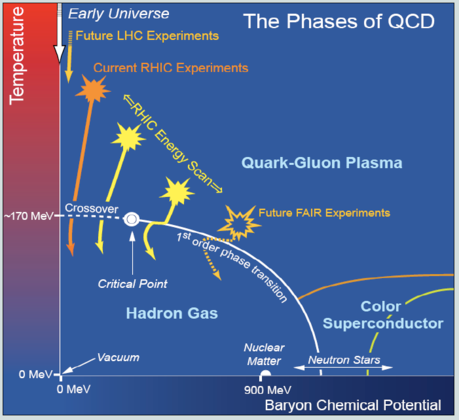
\includegraphics[width=0.45\textwidth]{Figures/Chapter1/QCDPhaseDiagram.png}
\caption{The theoretical QCD phase diagram of different QCD matter, including hadron resonance gas, quark-gluon plasma, neutron star, and color superconductor, as function of temperature and baryon chemical potential is shown above. The solid line indicates the conjecture of first order phase transition between quark-gluon plasma and hadron gas while the dash line is a smooth crossover.}
\label{QCDPhaseDiagram}
\end{center}
\end{figure} 

\subsection{Hadron Resonance Gas}

One of the most familiar type of QCD matter is hadron resonance gas, which lies at the left bottom corner of the QCD phase diagram. Hadron resonance gas is a system of color neutral hadrons at relative low temperature. The interaction between hadrons are the Van der Waas like strong nuclear force as the residue of the color force via exchange of mesons. The strong nuclear force between two nucleons shown below Figure \ref{NuclearForce}. 

\begin{figure}[hbtp]
\begin{center}
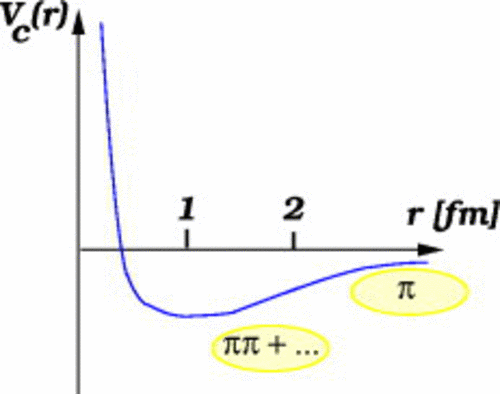
\includegraphics[width=0.45\textwidth]{Figures/Chapter1/NuclearForce.png}
\caption{The schematic plot of potential energy between two nucleon via pion exchange as a function of distance is shown above \cite{StrongNuclear}. This potential with a well minimizing near 100 MeV allow nucleons to bind together and form atomic nuclei and nuclear matter.}
\label{NuclearForce}
\end{center}
\end{figure} 

The equation of state of non-interacting hadron resonance gas could be described by grand canonical ensemble of bosons (mesons) and fermions (baryons) \cite{StatMechHadron}. We should note that pions dominates the hadron gas at low temperature. The realistic equation of state of hadron resonance gas should also consider the interaction. An example of the equation of state of hadron resonance gas consider the Van der Waas interaction comparing with lattice QCD simulation is given in Figure \ref{EOSHadronLattice} below \cite{EOSHadron}:

\begin{figure}[hbtp]
\begin{center}
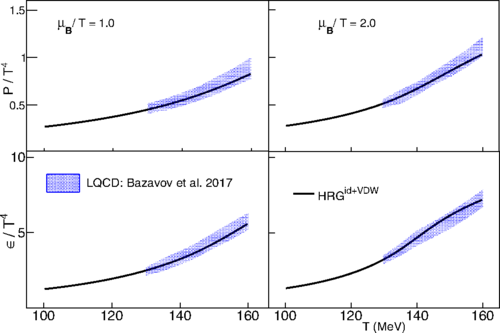
\includegraphics[width=0.45\textwidth]{Figures/Chapter1/EOSHadronGas.png}
\caption{The pressure and energy density from lattice simulation compared with ideal hadron resonance gas and Van der Waas interaction at different $\frac{\mu_B}{T}$ are shown above.}
\label{EOSHadronLattice}
\end{center}
\end{figure} 



Nuclear matter is considered as part of the hadron resonance gas in the QCD phase diagram. Examples of typical hadron gas will be atomic nuclei at a famous nuclear matter saturation density $n_S$ = 0.16 $fm^{-3}$ (baryon density $n_B = 3 n_S$) and nuclear matter like neutron star at large baryon density. 

\subsection{Quark-Gluon Plasma}

At very high temperature, quarks and gluons inside the color neutral hadron resonance gas will deconfine and form a new type of matter called quark-gluon plasma (QGP). In cosmology, it is believed that QGP exists in the early universe just several microseconds after the Big Bang during the quark epoch after electroweak phase transition and before nucleosynthesis \cite{QGPCosmology}. 



The temperature of QGP is in order of hundreds of MeV, which is about hundreds of thousands times hotter than the core of the Sun. Moreover, according to extensive experimental and theoretical studies, QGP demonstrates strongly coupled ideal liquid behavior, which directly contracts to the prediction from asymptotic freedom which predict such matter should behavior like a gas of weakly interacting quarks and gluons. Therefore, the inner workings and proper degrees of freedom of QGP must be somewhere in between weakly coupled quarks and gluons and color neutral hadrons because it still demonstrate significant color freedom due to deconfinement. However, the microscopic structure of QGP is still unknown. Currently, both experimental and theoretical efforts have been conducted to actively investigate the internal structure of QGP.

Based on its ideal liquid feature, QGP could be described by relativistic viscous hydrodynamics. In fact, the quantum limit predicted by the Anti-de-Sitter Space Conform Field Theory (AdS/CFT). It is about a factor of larger than water.

The accurate equation of state of QGP is currently unknown. However, it is safe to assume that the strong interaction dominates in the QGP phase because its large coupling results in large cross section compared to the electroweak interaction cross section. Therefore, one can consider only strong interaction between quarks and gluons in the QGP. According to MIT Bag Model, the energy density $\epsilon$ and pressure $p$ of a plasma of free quarks and gluons as a function of temperature $T$ is as follows \cite{MITBag}:

\begin{equation}
\epsilon = \frac{37 \pi^2}{30} T^4 + \mathcal{B}
\end{equation}

\begin{equation}
p = \frac{37 \pi^2}{90} T^4 - \mathcal{B}
\end{equation}

Here, $\mathcal{B}$ is the Bag Constant, which can be understood as the pressure of the vacuum on the quarks and gluons to make them form hadrons with finite size.

If we represent $p$ in terms of $\epsilon$, we get

\begin{equation}
p = \frac{1}{3} (\epsilon - 4\mathcal{B})
\end{equation}

Figure \ref{QGPEOS} below shows the equation of state of QGP of three flavor quarks of different model at $\mu_B = 0$ \cite{QGPEOSRef}. 


\begin{figure}[hbtp]
\begin{center}
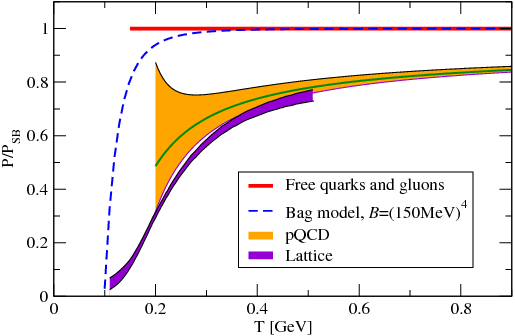
\includegraphics[width=0.60\textwidth]{Figures/Chapter1/QGPEOS.png}
\caption{Predictions the normalized pressure to the stefan Boltzmann pressure $P_{SB} = \sigma T^4$ as a function of temperature $T$ for three-flavor QGP obtained from lattice QCD, the MIT bag model and perturbative QCD including their uncertainties bands are shown.}
\label{QGPEOS}
\end{center}
\end{figure} 

We can clearly see that a gradual rise of the pressure from near 0 to 1 as the temperature increases, indicating an smooth increase the total degree of freedom of the system due to the color deconfinement. 


\subsection{Color Superconductor}

Under extremely high net baryon density, there is another hypothetical state of QCD matter named Color Superconductor where the color charges can move freely \cite{ColorSuperconductor}. Similar to the Cooper Pair formation mechanism of electrons in metals, quarks, as fermions, pair up and bosonized into diquark, and undergo Bose-Einstein condensation \cite{ColorSuperconductor}. The diquark condensate, carrying color charges, can move without resistance and thus demonstrate color superconductivity. It is believed that the color superconductor exists in the core of neutron stars where the net baryon chemical potential is high \cite{CSCOccurrence}. However, so far no color superconductor has been discovered in laboratory or astrophysical observations. 

\subsection{Phase Transition}

As we increase the temperature, hadron resonance gas will undergo a phase transition into QGP. The chiral symmetry is restored from the phase transition of hadron resonance gas to QGP. However, the order of the phase transition from resonance hadron to QGP is still unknown. According to lattice QCD calculations, near zero baryon chemical potential ($\mu_B = 0$), the phase transition is a smooth cross over. According to lattice QCD calculations, at $\mu_B = 0$, the degree of freedom transition drastically increases near the critical temperature $T_c$. 

 

 However, at finite baryon chemical, it is believe that the phase is a first order phase transition according to different model calculations \cite{QCDFirstOrder}. The hint of first order phase transition can be found in the softening equation of state in the cross over region \cite{EOSPhase}. However, currently, the order of phase transition from hadron resonance gas to QGP at high baryon chemical potential is still an open question. %However, there is no direct physical observable to determine the order of the phase transition in experiments \cite{Observables}.

\subsection{Critical Point}

If the theoretical predictions are correct, according to thermodynamics, there must be a critical point between the first order phase transition and the smooth crossover. Theoretical calculations predict that the critical point is $\mu_B = $ 350 -- 700 and $T_{c}$ $\approx$ 160 MeV \cite{CriticalPointTH}. Experimentally, the scale of the critical temperature may occur at $T_{c}$ $\approx$ 175 MeV from high moment analyses \cite{CriticalPointEX}. The research on critical point, a landmark in the QCD phase diagram, and the phase transition between QGP and hadron resonance gas are very important topics for physicists to understand the nature of QCD matters. The STAR Collaboration has carried out a Beam Energy Scan, both Phase I and II, at RHIC and plan to extend it to higher baryon chemical ponetial and lower temperature in the future Fixed Target Mode to search the critical point in the QCD phase diagram. However, so far efforts to search the precise locations of the critical point is still ongoing. The results are still inconclusive \cite{STARBES}. 

\section{High Energy Nuclear Physics}

Nuclear Physics is a study of atomic nuclei and their structures and interactions, which a typical energy scale ranging from MeV to GeV. High Energy Nuclear Physics is a subfield of Nuclear Physics at an energy scale on the order of GeV using heavy nuclei (A > 56). Its main goal is to under the physics of QCD matter from various approaches such as collider experiments, astrophysical observations, lattice QCD computation, and theoretical modeling. In this thesis, I will focus on the research of QGP physics from the experimental approach using high energy heavy-ion colliders.

\subsection{Laboratories}

In laboratories, high energy nuclear physicists accelerate and collide heavy ions (A > 56) at center of mass high energy per nucleon at grater than 1 GeV to create extremely hot and dense condition and study QGP. Relativistic heavy-ion collision is also known as ``The Little Bang'' compared to ``The Big Bang'' in cosmology \cite{}. Historically, many colliders, such as the Alternating Gradient Synchrotron (AGS) at Brookhaven National Laboratory (BNL), in Upton, Long Island, New York and Super Proton Synchrotron (SPS) at European Center for Nuclear Research (CERN) in Meyrin, Switzerland, and GSI at Helmholtz Centre for Heavy Ion Research with both proton-proton and relativistic heavy-ion collision capabilities, have been built and established high energy nuclear physics research programs. Today, two active colliders, the RHIC at BNL and LHC at CERN, are running at different energy with various nuclei species at a wide range of impact parameters. In the future, another one collider Facility for Antiproton and Ion Research (FAIR) running at a relatively low energy and high baryon chemical potential is being constructed at Darmstadt, Germany to map the location of critical point in the QCD Phase Diagram. 

In addition to collider facilities, QGP might also be studied from astrophysical observations. For instance, strange stars, a quark star made of strange quark matter, may be form from stable strangelet according to Bodmer--Witten conjecture \cite{SQMReview} or exist in the core of neutron stars under extreme pressure and temperature. It is believe there are several potential strange stars candidates according to telescope observations and gamma ray burst analysis \cite{SS1,SS2,SS3}.

%\subsection{Heavy-Ion Accelerators}

\subsection{Relativistic Heavy Ion Collider (RHIC)}

Located at BNL in Upton, Long Island, New York, United States of America, RHIC is one of the major high energy accelerator facilities and currently the highest energy collider in America. It is a circular collider with a circumference of 3.843 kilometers and can provide proton energy up to 500 GeV and gold energy up to 200 GeV \cite{RHICReport}. It was built in 2000 in order to search for a strongly interacting hot and dense state of matter created under ultra-relativistic heavy-ion collisions, currently known as QGP, with hints from the measurement at AGS. Moreover, RHIC provides physicists with a wide range of energies and a variety of ion species from proton to deuteron and cooper to uranium create different sizes of system at different temperature and baryon chemicals. In addition, taking the advantage from its highly polarization beam with high luminosity, it has a great machine capabilities for cold QCD physics. Figure \ref{RHIC} below shows a sky view of RHIC at BNL:


\begin{figure}[hbtp]
\begin{center}
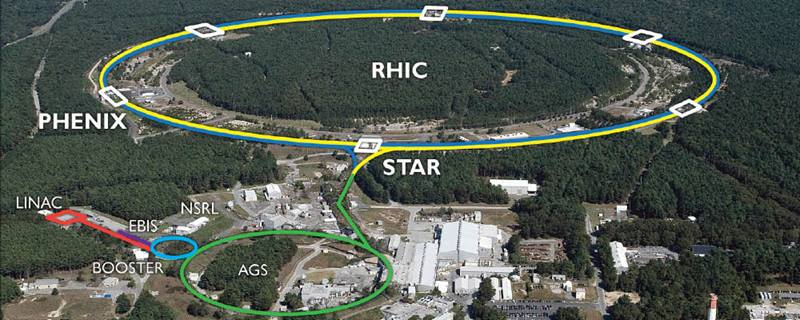
\includegraphics[width=0.85\textwidth]{Figures/Chapter1/RHIC.jpg}
\caption{The overview of RHIC at BNL from the sky view is shown above. The actual locations of other accelerator facilities at BNL, including Linac, Booster, EBIS, NSRL, AGS, and the experiments at RHIC,STAR and PHENIX, are also labelled.}
\label{RHIC}
\end{center}
\end{figure} 

Here is how RHIC accelerates charged particles to the energy scale of GeV per nucleon. For instance, if we consider the acceleration of a typical ion source gold (${}^{197}_{79}Au$) ion, we first use a cesium sputter ion source operated in the pulsed beam mode point to the gold metal and produce the $Au^-$ ion \cite{FirstAuSource}. Then, the $Au^{-}$ will undergo a series of electron stripping process to reach the $Au^{79+}$ ion \cite{RHICStrpDetail}. First, 13 electrons are stripped by the carbon foil in the Terminal Stripping (S1) after the acceleration of tandem Van der Gaaf generator to turn $Au^{-}$ to $Au^{12+}$. Then, the $Au^{12+}$ ion will go through the Object Foil (S2) at the second stripping stage and becomes $Au^{31+}$. Next, the $Au^{31+}$ will go through the third stripping station BTA foil (S3) made of aluminum and vitreous carbon between the Booster Synchrotron and AGS and becomes $Au^{77+}$. Finally, two more electrons of the gold ion $Au^{77+}$ are removed at the fourth stripping station ATF foil (S4) made of thin tungsten, located between the AGS and RHIC. The fully stripped gold ion $Au^{79+}$ inject to the blue and yellow rings at RHIC. For polarized protons, $H^-$ pass a single stripping stage called located in the Booster Synchrotron. The stripping station is called Linac-to-Booster (LTB) stripper made of carbon foils with special geometry and converts polarized $H^-$ to $H^+$. Figure \ref{AccAu} schematically shows the accelerating process of gold ions at RHIC \cite{AuStripRef}

\begin{figure}[hbtp]
\begin{center}
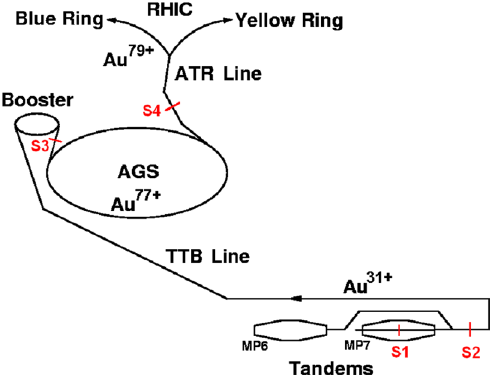
\includegraphics[width=0.45\textwidth]{Figures/Chapter1/AccAu.png}
\caption{The acceleration of gold ions for RHIC is shown above.}
\label{AccAu}
\end{center}
\end{figure} 

At RHIC, we will accelerate the $Au^{79+}$ ions in the superconducting Radio Frequency (RF) cavity under perpendicular electric and magnetic fields and increase their energies to about 100 GeV/c per nucleon. Then, we collider them via bunch crossing at interaction points of the experiments to perform relativistic heavy-ion collisions to study high energy nuclear physics. The RHIC collider usually operates in the first six months of a calendar year. At RHIC, the energy can also be lower where the ion beam collides with ions at a lower energy in the laboratory frame. STAR beam energy scan even fixed target mode.

\subsection{Large Hadron Collider (LHC)} 

Located at the border between Switzerland and France, LHC is one of the major high energy accelerator facilities in Europe and currently the highest energy collider in the world. It is a circular collider with a circumference of 26.7 kilometers and can provide proton energy up to 14.0 TeV and lead ion energy up to 5.02 TeV \cite{LHCReport}. It was built in 2008 with the main purpose to discover the Higgs Boson, perform precision measurements on SM, and search for Physics beyond SM. Due to its high energy and ion capabilities, high energy nuclear physicists also use the existing general purpose detectors for high energy particle experiment at the LHC to conduct research on relativistic heavy-ion physics. LHC ion physics runs usually starts at the end of the year and lasts for about a month. The photo taken from the sky to picture LHC is shown in Figure \ref{LHC}:

\begin{figure}[hbtp]
\begin{center}
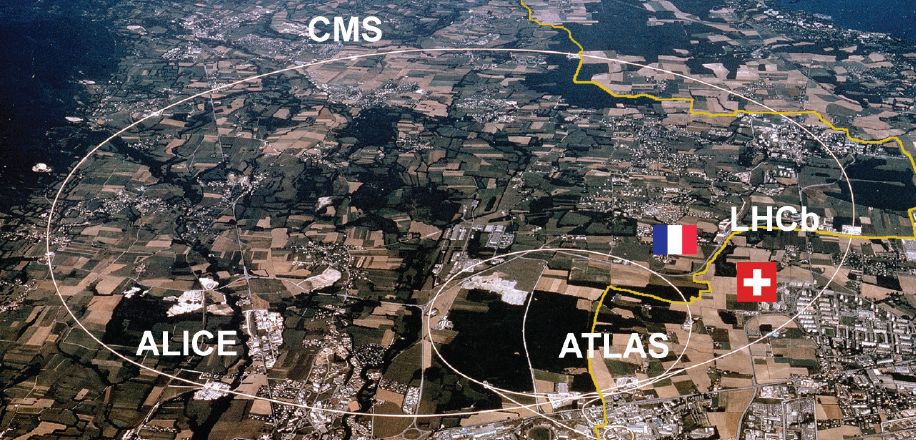
\includegraphics[width=0.85\textwidth]{Figures/Chapter1/LHC.png}
\caption{The overview of LHC at CERN from the sky view is shown above. The actual locations of the experiments at the LHC, ATLAS, CMS, ALICE and LHCb, as well as the French-Swiss border, are also labelled.}
\label{LHC}
\end{center}
\end{figure} 

The ion source CERN usually uses is lead ${}^{208}_{82} Pb$, which is stable and approximately spherical. In the 2017 ion run, it also used the xenon ${}^{131}_{52} Xe$. Currently, there is also a discussion of potential future lighter ions such as oxygen ${}^{32}_{16} O$ \cite{OORun}. Similar to RHIC, the lead ion at the LHC also undergoes a series of stripping processes using stripping foils in to order to become partially ionized $Pb^{81+}$ \cite{LHCStrip}. Also, the lead ions pass a series of energy boosting before reaching to the desired energy at the LHC. Lead ions starts from a source of vaporized lead and enter Linac 3 before being collected and accelerated in the Low Energy Ion Ring (LEIR) at the energy from 4.2 MeV to 72 MeV. Then, the lead ion will inject to Proton Synchrotron (PS) to boost its energy. Then, the they are sent to the Super Proton Synchrotron (SPS). Finally, the lead ion are injected to the LHC and increase their energy to TeV scale two LHC rings with the RF cavity with 400 MeV and an electric field strength of 5 MV/m \cite{LHCReport}. The energetic lead ions beams from two LHC rings will collide heads on with a small crossing angle at the interaction points of the LHC experiments. The CERN accelerator complex is shown schematically in \ref{CERNAccComplex} 


\begin{figure}[hbtp]
\begin{center}
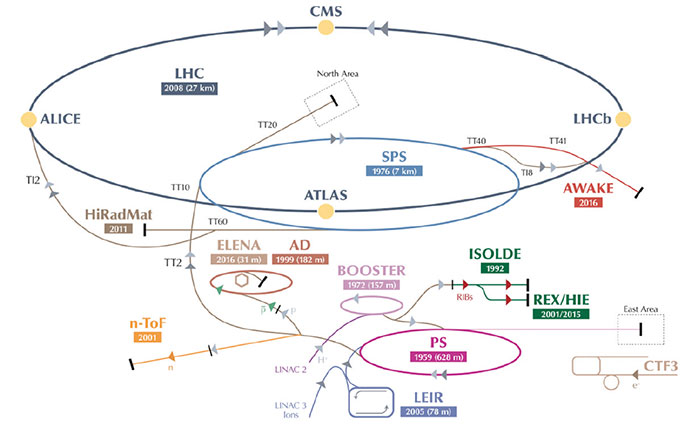
\includegraphics[width=0.65\textwidth]{Figures/Chapter1/CERNAccComplex.jpg}
\caption{The schematic overview of CERN accelerator complex with the accelerators labelled is shown above. Proton and lead ion are accelerated using these facilities to boost to the energy scale of TeV.}
\label{CERNAccComplex}
\end{center}
\end{figure} 

After Run III, LHC will upgrade to High Luminosity (HL) LHC and allow physicists to collect huge datasets, which is crucial for the precision measurements to study QGP in the heavy-ion physics program. Due to its far higher energy than RHIC, the QGP created at LHC has a higher temperature and a smaller baryon chemical potential than the one created at RHIC.  

\subsection{High Energy Physics Coordinates}

As mentioned in the previous section, the collision system of heavy-ion is in general highly relativistic. Therefore, Lorentz transformation will be relevant in our studies. In Cartesian coordinates $x^\mu = (t,x,y,z)$, under Lorentz transformation, if we boost the system by a speed $\beta$ in the $+z$ direction. The Lorentz gamma factor will be given by $\gamma = \frac{1}{\sqrt{1 - \beta^2}}$. The four vector $x^\mu \rightarrow x'^\mu$ transforms as follows

\begin{align}
   \begin{bmatrix} 
           t' \\
           x' \\
           y' \\
           z' \\
         \end{bmatrix} =
             \begin{bmatrix} 
             \gamma  & 0  & 0 & - \gamma \beta \\ 
            0 & 1 & 0 & 0 \\ 
             0 & 0 & 1 & 0 \\
             - \gamma  \beta & 0 & 0 &  \gamma \\
	\end{bmatrix} 
	  \begin{bmatrix} 
           t \\
           x \\
           y \\
           z \\
	\end{bmatrix}
\end{align}

The equation above is called the Lorentz Transformation. It is an orthogonal transformation preserving the Minkowski metric tensor $diag(1,-1,-1,-1)$ using particle physicists conventions.



Experimentally, nowadays, heavy-ion detectors usually have $2\pi$ angular coverage in the transverse direction with some finite longitudinal acceptance along the beam line. They look cylindrically symmetric. Hence, it is convenient and wise to choose a cylindrical coordinate system and use kinematic variables with Lorentz invariance, including boosting and rotation. In standard cylindrical coordinates in the position space, Lorentz four-vectors is used $(t,x,y,z) \rightarrow (t, r, \phi, z)$. 


The relativistic coordinate system for our analysis are shown below in Figure \ref{HICoordinates}. 

\begin{figure}[hbtp]
\begin{center}
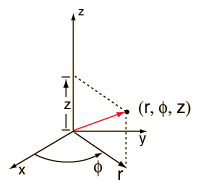
\includegraphics[width=0.40\textwidth]{Figures/Chapter1/PosCylindrical.png}
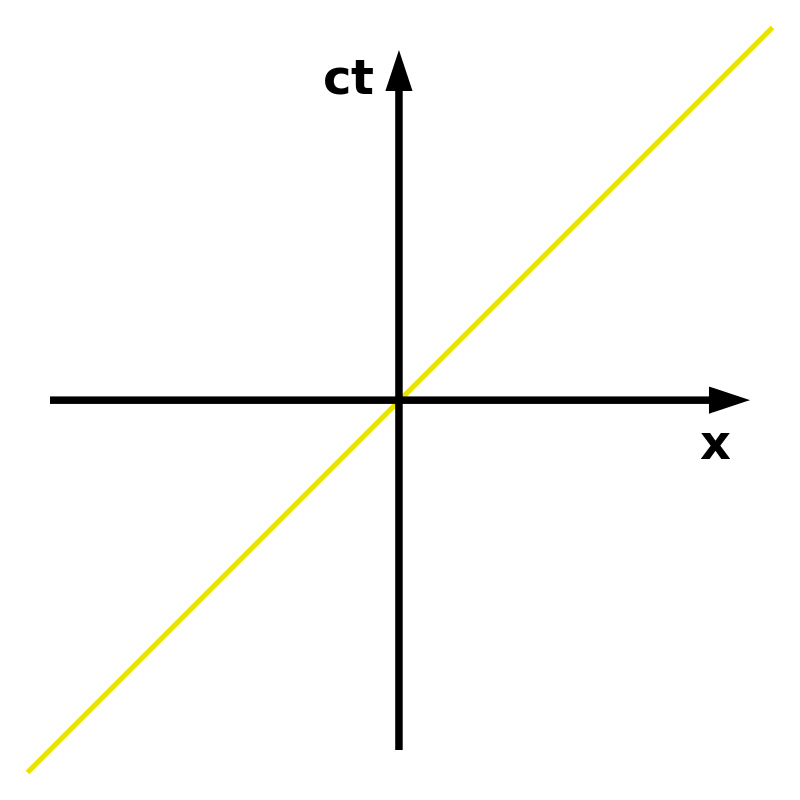
\includegraphics[width=0.40\textwidth]{Figures/Chapter1/STDiagram.png}
\caption{The cylindrical coordinate system in the position space (left) and the space time diagram (right) for relativistic heavy-ion physics analysis are shown above.}
\label{HICoordinates}
\end{center}
\end{figure} 


Thus, for the momentum space, we can use $p^\mu = (E,p_x, p_y, p_z) \rightarrow  (E,p_T, \phi, p_z)$ 

\begin{equation}
p_T = \sqrt{p_x^2 + p_y^2}
\end{equation}

\begin{equation}
\phi = \arctan(\frac{p_y}{p_x})
\end{equation}

We also define rapidity $y$, a relativistic version of velocity that can be convenient add to the boost.

\begin{equation}
y = \frac{1}{2} \ln \frac{E+p_z}{E-p_z}
\end{equation}


Experimentally, we also use pseudo-rapidity $\eta$, which is more directly connected to the detector measurement assuming ultra-relativistic limit kinematics ($E \rightarrow p$). The definition of pseudo-rapidity $\eta$ is shown as follows:

\begin{equation}
\eta =  - \ln \tan(\frac{\theta}{2})
\end{equation}

Here $\theta$ is the angle labelled in the left of Figure \ref{HICoordinates}. Particularly, $y = 0$ and $\eta = 0$ when $p_z = 0$. In addition, boosting by a speed $\beta$ in the longitudinal z-direction, we found that the rapidity simply shift by a const number $y' = y + \tanh \beta$. We should note that the cylindrical coordinates ($p_T$,$\phi$, $p_z$) are perfectly orthogonal while ($p_T$,$\phi$, $y$) or ($p_T$,$\phi$, $\eta$) are not.

For general collider experiments, two particles are moving toward each other with four-momenta $p_1^\mu$ and $p_2^\mu$ and interact with each other. It is also very convenient to use the Mandelstam variables $s, t, u$ in our studies. They are defined as follows

\begin{equation}
s \equiv (p_1 + p_2)^2
\end{equation}

\begin{equation}
t \equiv (p_1 - p_2)^2
\end{equation}

\begin{equation}
u \equiv (p_1 - p_3)^2
\end{equation}


Here the center of mass frame, since we know the tree vector $\vec{p_1} = -\vec{p_2} = \vec{p}$ energy is the Mandelstam variable $s \equiv (p_1 + p_2)^2$ where $p_1$ and $p_2$ are the four-momenta of the incident beam particles. Therefore, we can see that $p_1^\mu = (E, \vec{p})$ and $p_2^\mu = (E, -\vec{p})$. Hence, $s \equiv (p_1 + p_2)^2$ = $4E^2$ = $E_{CM}^2$. Hence, the center of mass energy of the collision system could be represented by the Mandelstam variable $\sqrt{s}$: $E_{CM} = \sqrt{s}$.


%\subsection{Heavy-ion Physics Detectors}

\subsection{Stages of Heavy-Ion Collisions}

In high energy heavy-ion collisions, both Electroweak and QCD processes occur in each event and contribute to the total cross section. We classify the events with elastic and inelastic reaction processes. For elastic processes, two nuclei scatter mainly electromagnetically with each via photon exchange without breaking themselves up or losing energy. For inelastic scattering, we classify diffractive and non-diffractive disassociation processes. In diffractive dissociation processes, the two nuclei may be slightly excited and lose a relatively small fraction of energy, producing relatively small number of particles. On the other hand, in non-diffractive dissociation processes, the nuclei lose a substantial fraction of their energies and produce a large number of particles \cite{CYWong}. 

Therefore, in events with significant contribution from non-diffractive dissociation, the interaction between two nuclei is indeed a multi-stage process including both perturbative and non-pertubative QCD processes. We can define stages of heavy collisions and understand the details of each stage. It consists of five stages: initial state of two high Lorentz contracted nuclei before the collision, the very early pre-equilibrium stage where hard scattering between partons inside nuclei starts, the rapid expansion of the fireball begins when the thermally and chemically equilibrated QGP, the hadronization stage after QGP expands and cools down, and the freeze-out stage when the inelastic scattering process ceases.


\begin{figure}[hbtp]
\begin{center}
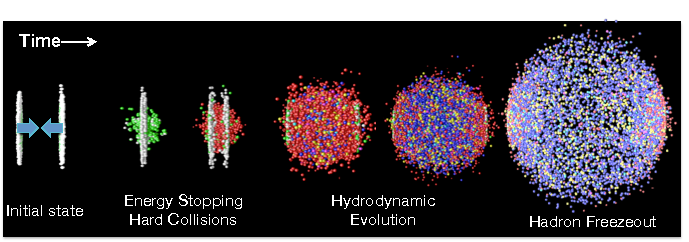
\includegraphics[width=0.75\textwidth]{Figures/Chapter1/Heavy-Ion-Process.png}
\caption{An event of a typical heavy-ion collisions event with different stages as time evolves is shown above.}
\label{CERNAccComplex}
\end{center}
\end{figure} 

\begin{figure}[hbtp]
\begin{center}
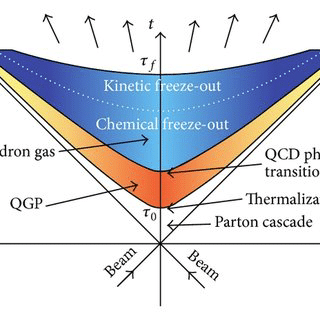
\includegraphics[width=0.45\textwidth]{Figures/Chapter1/HICSTEvolve.png}
\caption{The space-time evolution of heavy-ion collisions is shown above. It consists of four stages: initial state before the collision, the creation of quark-gluon plasma right after of the collision, hadronization after quark-gluon plasma expands and cools down, and the freeze-out stage, first chemical freeze out when the particle species no longer change, and then kinetic freeze out when the inelastic scattering process ceases.}
\label{CERNAccComplex}
\end{center}
\end{figure} 

Theoretically, many phenomenological models such as Ultra-Relativistic Quantum Molecular Dynamics (UrQMD) and A Multi-Phase Transport Model (AMPT) are developed to describe relativistic heavy-ion collisions. 


\subsection{Global Event Observables}

Globally, we can define some physics quantities to describe heavy-ion collisions to generally characterize each event. Heavy-ion Physicists defined the impact parameter, centrality, number of participants, We will discuss all of them below.

\textbf{Impact Parameter:} Prior to heavy-ion collisions, similar to other collider experiments, each event are prepared with the same unpolarized incoming particles with the same center of mass energy. Therefore, the incoming state $\ket{i}$ is used for each event. However, different from $e^+ e^-$ and $pp$ collision, in heavy-ion physics, we introduce another parameter called the impact parameter denoted $b$ to the transverse distance between center of two nuclei to classify the events. Therefore, the incoming state can be rewritten as  $\ket{i (b)}$. Figure \ref{IPHIColl} shows the definition of impact parameter in heavy-ion collision \cite{IPHICText}.

\begin{figure}[hbtp]
\begin{center}
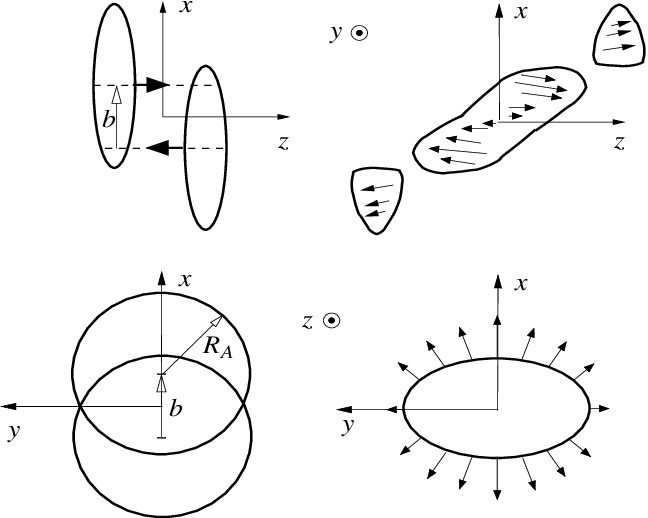
\includegraphics[width=0.45\textwidth]{Figures/Chapter1/IPHIColl.png}
\caption{The definition of impact parameter $b$ in heavy-ion collision and the of overlapping interaction region and the break up remnants of the two nuclei, which is called spectator, moving in the z-direction are shown above. We can also see that heavy-ion collisions have an almond shape interaction region, which results in the azimuthal anisotropic emission of final state particles.}
\label{IPHIColl}
\end{center}
\end{figure} 


\textbf{Number of Participating Nucleons:} Right at the end of heavy-ion collisions after two nuclei pass through with each other, we can define the number of participating nucleon denoted $N_{part}$. The smaller the impact parameter, the more overlap volume between two nuclei, leading to a larger number of number of participating nucleon in the collision. The nuclear interaction system size is determined by the number of participating nucleons. However, due to event-by-event nuclei geometry fluctuations caused by the motion of nucleons inside nuclei \cite{GuntherV3}, it is more proper to say that the average number of participating nucleon is related to the impact parameter.

\textbf{Number of Binary Nucleon-Nucleon Collisions:} In addition to $N_{part}$, we can also define another quantity that characterize details interaction of the events at the rather hard scale. The number of binary nucleon-nucleon collisions, denoted $N_{coll}$, is also related to the impact parameter. At higher energy, nucleons inside nuclei become a relevant degree of freedom to the cross section. We could treat the collisions of two nuclei as the superposition of the collisions between nucleons inside the nuclei. Since binary nucleon-nucleon collision has a rather small cross section, it dominates the total nucleon-nucleon cross section according to binomial principle. Glauber model is developed to study the relationship between $b$, $N_{part}$, and $N_{coll}$ in nuclei collisions and will be discussed in the following subsection.


\textbf{Centrality:} Experimentally, it is difficult to directly measure the impact parameter of each collision. Therefore, we define another physical quantity called centrality to characterize the impact parameter. The centrality ($C$) is defined fraction of the total nuclear interaction cross section: $C = \int^b_0 \frac{d\sigma}{dx} dx$ . Centrality is expressed in terms of percentage \cite{CentDef}. It is proportional to the quantity: $\frac{\pi b^2}{4\pi R_A^2}$ where $R_A$ is the radius of a nuclei defined above in Figure \ref{IPHIColl}. When the impact parameter between two nuclei is 0, the centrality is at 0\%. When the  impact parameter between two nuclei is 2$R_A$, the centrality is 100\%. There is a relationship between the centrality and the average number of participant nucleons. Heavy-ion experimental measurements are in general presented in terms of centrality or average number of participating nucleon. Experimentally, we look at the number of tracks and activities of calorimeters at the very forward direction (Zero Degree Calorimeters) to estimate the centrality \cite{ALICEZDC,CMSZDC,ATLASZDC}. 


\textbf{Virtuality:} Similar to deep inelastic scattering, we can also define the virtuality $Q^2$, which is the momentum transfer between the two nucleons in nucleon-nucleon collisions. To generate nucleon-nucleon collision event, we used $\hat p_T$, defined as the transverse momentum of the hard subprocess, which is a quantity related to $Q^2$, developed by the high energy theory group of Lund University.



\textbf{Event Multiplicity:} We can also define the event multiplicity by counting the number of final state charged particles to quantify the activity of the event. Event multiplicity can be denoted as $N_{trk}$, number of tracks in the event, which is proportional to the number of charged particle denoted as $N_{ch}$. Figure \ref{CentDefPlot} shows the correlation between the number of participating nucleons in a heavy-ion collision, their cross section and the impact parameter, defining the centrality classes \cite{CentPlot}.


\begin{figure}[hbtp]
\begin{center}
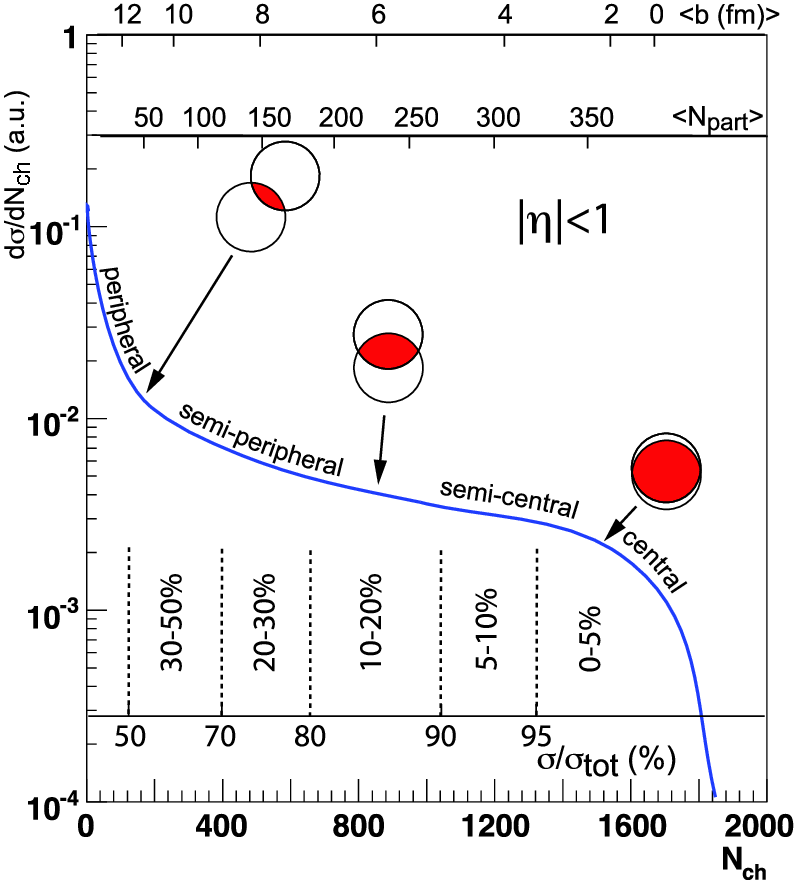
\includegraphics[width=0.45\textwidth]{Figures/Chapter1/CentDefPlot.png}
\caption{The plot showing relationship among number of charged particle, $N_{ch}$, related to the number of participating nucleon $N_{part}$, the differential cross section $\frac{d\sigma}{dN_{ch}}$, and the centrality, according to the Glauber Model calculations, is shown above.}
\label{CentDefPlot}
\end{center}
\end{figure} 


The initial global parameters such as the collisions energy, impact parameter, and polarization can be treated the knobs for high energy nuclear physicists to play with in order to study relativistic heavy-ion collisions and create the strongly interacting system at different sizes with different chemical potentials and temperatures in the QCP phase diagram. Figure \ref{STAREvtDisplay} shows an event display of thousands of tracks from a central Au + Au collision event at 200 GeV recorded by the Time Projection Chamber (TPC) of the STAR experiment at RHIC.


\begin{figure}[hbtp]
\begin{center}
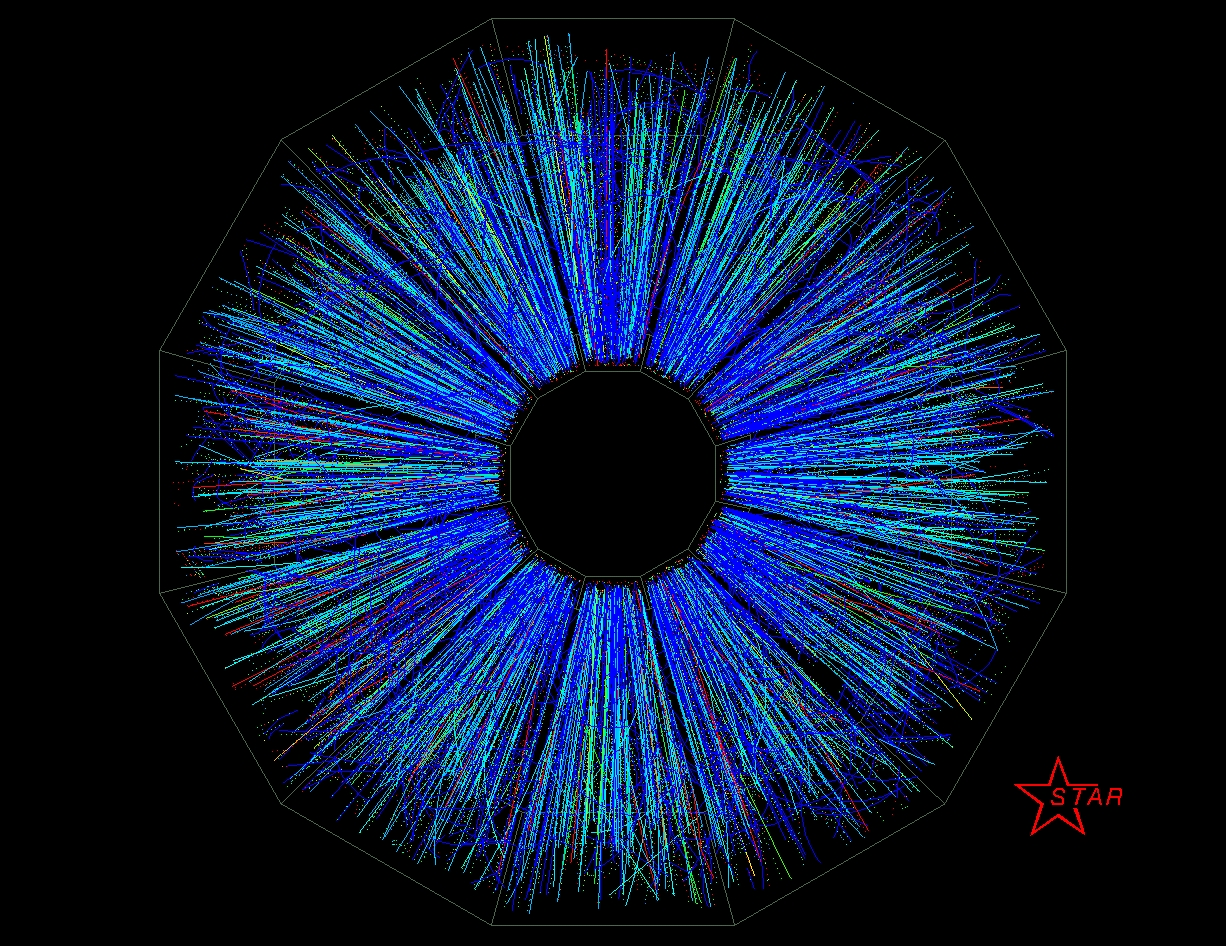
\includegraphics[width=0.50\textwidth]{Figures/Chapter1/STAREvtDisplay.png}
\caption{Two gold ions collide head-on in the STAR detector. The event with reconstructed tracks of final state particles are display by STAR TPC shown above.}
\label{STAREvtDisplay}
\end{center}
\end{figure} 



\subsection{Glauber Model}

The Glauber Model, named after Physicist Roy Glauber \cite{Glauber}, is originally developed to address high energy scattering problem with composite particles in the optical limit where optical theorem is applicable \cite{Optical1,Optical2}. It is a model describing two composite objects collider inelastically with each other and relate the cross section to the cross section of collision between two point objects. The Glauber Model can be applied to study nucleon-nucleus (N-A) and nucleus-nucleus (A-B) collisions with nucleon-nucleon (N-N) collisions and determine relationship between the global observables mentioned in the previous subsection.    

 If we consider a spherically symmetric nucleus, the nuclear charge density can be parameterize $\rho(r)$ by the Fermi distribution with three parameters below

\begin{equation}
\rho(r) = \rho_0 \frac{1 + w(r/R)^2}{1 + \exp({\frac{r-R}{a}})}
\end{equation}

According to the Glauber Model \cite{Glauber}, the N-N inelastic cross section is denoted as $\sigma_{in}^{NN}$ and the effective thickness function of a nucleon is defined as a function of impact parameter in the transverse direction: $T(\vec{b})$. It is defined as follow

\begin{equation}
T(\vec{b}) =  \int \rho(\vec{b},z) dz 
\end{equation}

It is normalized to unity: $\int^{R_A}_0 T(\vec{b}) d^2b = 1$. $T(\vec{b})$ essentially depends on density of the nucleus $r(b)$. If the nucleus has a uniform cylinder and the collide on its circular face along its height, then $T(\vec{b})$ will be a constant. Therefore, the probability that a nucleon collides with a nucleon inside the nucleus is given by $\sigma_{in} T(\vec{b})$. Therefore, the probability of $n$ nucleon collision is given by

\begin{equation}
P_n = {A \choose n} \sigma_{in}^{NN} T(\vec{b})^{n} [1 - \sigma_{in} T(\vec{b})]^{A-n}
\end{equation}

Hence, if we consider a constant fraction of $\mu$ ($0 \le \mu \le 1$) of particle produced after each collisions, we can calculation the average multiplicity $\langle N(\mu) \rangle$:

\begin{equation}
\langle N(\mu) \rangle = \Sigma_n P_n \Sigma^{n-1}_0 \mu^m =  \Sigma_{n-1} P_n \frac{1 - \mu^n}{1 - \mu} = \frac{1}{1-\mu} \{ 1 - [1 - (1-\mu) \sigma_{in} T(\vec{b})]^A \}
\end{equation}

It turns out that we have the following relationship between $N_{part}$ and $N_{coll}$ with $\langle  N(\mu) \rangle$  \cite{Glauber}

\begin{equation}
N_{part} = \langle N(\mu = 0) \rangle 
\end{equation}

\begin{equation}
N_{coll} = \frac{1}{2} \langle N(\mu = 1) \rangle = A T(\vec{b}) \sigma_{in}^{NN}
\end{equation}

In a more generalized case: A-B collisions, Figure \ref{GlauberRef} shows sides view and beam-line view of heavy-ion collision of projectile B on target A


\begin{figure}[hbtp]
\begin{center}
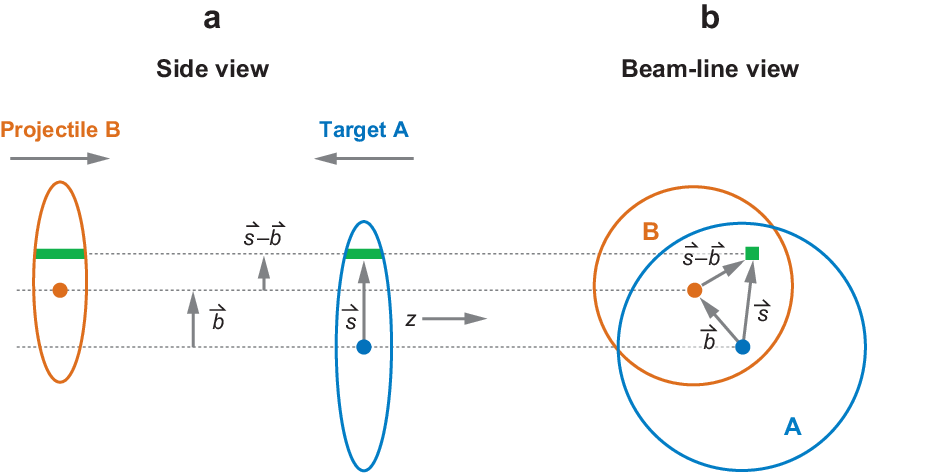
\includegraphics[width=0.65\textwidth]{Figures/Chapter1/GlauDefColl.png}
\caption{The A-B collision with the definition of the impact parameter vector $\vec{b}$ and the distance of nucleon to the center of projectile B $\vec{s}$ are shown above. The distance of the nucleon in B to center of the target A is $\vec{s}-\vec{b}$ according to vector subtraction rule. Here we assume both nuclei A and B are perfect spheres.}
\label{GlauberRef}
\end{center}
\end{figure} 

Using similar ideas \cite{CentPlot}, we could first calculate the effective thickness function $T_{AB}$ as follows:


\begin{equation}
T_{AB}(\vec{b}) = \int T_A(\vec{s}) T_B(\vec{b} - \vec{s}) d^2s 
\end{equation}



Now replacing T($\vec{b}$) in N-A by $T_{AB}(\vec{b})$ in A-B, we can obtain

\begin{equation}
\langle N(\mu) \rangle = \frac{A}{1-\mu} \int_0^b T_A(\vec{s}) \{1 - [1 - (1 - \mu) T_{B}(\vec{b}-\vec{s}) \sigma_{in}^{NN}]\}^A d^2s  +  \frac{B}{1-\mu} \int_0^b T_B(\vec{s}) \{1 - [1 - (1 - \mu) T_{A}(\vec{b}-\vec{s}) \sigma_{in}^{NN}]\}^B d^2s
\end{equation}


To obtain $N_{part}$, evaluate at $\mu = 0$, we get 

\begin{equation}
N_{part} =  A \int_0^b T_A(\vec{s}) \{1 - [1 - T_{B}(\vec{b}-\vec{s}) \sigma_{in}^{NN}]^A\}d^2s +  B \int_0^b T_B(\vec{s}) \{1 - [1 - T_{A}(\vec{b}-\vec{s}) \sigma_{in}^{NN}]^B\} d^2s
\end{equation}

To obtain $N_{coll}$, evaluate at $\mu = 1$, we get

\begin{equation}
N_{coll} = AB T_{AB}(\vec{b}) \sigma_{in}^{NN}
\end{equation}

In a very special case, assume the nucleon are simply perfect rigid sphere with the same radius and head-on collide with each other (impact parameter is $b=0$). That is $T_{A} \sigma_{in}^{NN} = T_{B} \sigma_{in}^{NN} = T_{AB} \sigma_{in}^{NN} = 1$, we get 


\begin{equation}
N_{part} = A + B
\end{equation}

\begin{equation}
N_{coll} = AB
\end{equation}

The results above of $N_{part}$ and $N_{coll}$ agree to our expectation. 

The comparison of the Glauber Model with simulations of the $N_{part}$ and $N_{coll}$ as a function of impact parameter $b$. Figure \ref{NPartandNColl} from the \cite{CentPlot}

\begin{figure}[hbtp]
\begin{center}
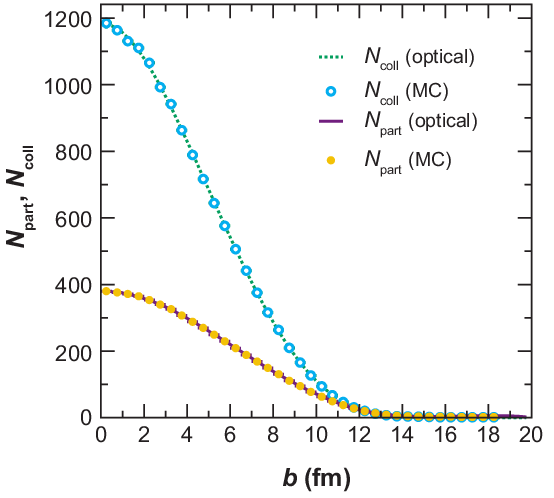
\includegraphics[width=0.50\textwidth]{Figures/Chapter1/NPartandNColl.png}
\caption{The $N_{part}$ and $N_{coll}$ as a function impact parameter calculated from the Glauber Model with optical approximation (lines) and from MC simulations (circles) are shown above. We can see they have almost perfect agreement with each other.}
\label{NPartandNColl}
\end{center}
\end{figure} 


Therefore, we can apply the Glauber model to determine $N_{part}$ and $N_{coll}$ for a given centrality range of AA collision ($T_{AB} \rightarrow T_{AA}$), which will be used in our analysis to obtain the corrected yield. It is believed that the production of light hadrons, such as pions and kaons, are scaled as $N_{part}$ \cite{NPartScaling} while electroweak bosons, such as W and Z boson, are scaled as $N_{coll}$ \cite{NCollScaling}.

\section{Characterization of Quark-Gluon Plasma}

Equipped with the knowledge and collider technologies of heavy-ion collisions, we are ready to apply them to conduct scientific research on QGP in laboratories. The following subsections will describe the characterization of QGP from its predicted signature to open questions today, which leads to my thesis research.

\subsection{Signatures}

QGP has been hypothesize long before its discovery as a color deconfined phase of quark matter named ``quark gluon plasma'' \cite{LeonQGP} and will demonstrate some specific benchmarks in experiments to prove the creation of QGP \cite{QGPSignature}. Here, four classic signatures of QGP will be discussed: $J/\psi$ suppression, jet quenching, elliptic flow, strangeness enhancement.  

\subsection{$J/\psi$ and $\Upsilon$ suppression} 

$J/\psi$ meson, as a type of heavy quarkonia, is bound state of $c\bar c$, made of charm quark and an anti-charm quark, whose mass is heavier than the $\Lambda_{QCD}$. Therefore, we could approximately treat the interaction between charm and the anti-charm quark a static the Cornell potential V(r) in the non-relativistic quantum mechanical hamiltonian system \cite{QuarkoniaV}: 

\begin{equation}
\hat H = \hat T + \hat V
\end{equation}

\begin{equation}
\hat H \ket{\psi} = i \frac{\partial}{\partial t}  \ket{\psi} 
\end{equation}

and solve Schrodinger equation the to describe $J/\psi$ mesons in vacuum \cite{}. As we have seen in Section 1.3.4, with the QGP medium, at a finite temperature $T$, the potential is modified due to color screen effect. As the distance between two charm quarks $V(r) \rightarrow \frac{\sigma}{m_D}$, which does not diverge, as $r \rightarrow \infty$. Therefore, the $c \bar c$ system could be unbounded if they have sufficient energy. In the field theory picture, this could be understood as the color string breaking between charm and anti-charm quark \cite{CSBQQ}, also known as quarkonia melting \cite{QQMelt}. Hence, with the influence of QGP at $T > 0$, the production cross section of $J/\psi$ will decrease compared to the vacuum at $T=0$. Experimentally, we define an observable to quantify the modification of particle production cross section in AA collision compared to the reference pp collisions normalized by the number of binary nucleon-nucleon collisions $N_{coll}$, which is defined in the previous subsection. We called this observable as nuclear modification factor denoted $R_{AA}$. Mathematically, $R_{AA}$ is defined as follows:

\begin{equation}
R_{AA} =\frac{1}{N_{coll}} \frac{\frac{d^2N_{AA}}{dp_T dy}}{\frac{d^2N_{pp}}{dp_T dy}} = \frac{1}{T_{AA}} \frac{\frac{d^2N_{AA}}{dp_T dy}}{\frac{d^2\sigma_{pp}}{dp_T dy}}
\end{equation}

Therefore, $R_{AA} < 1$ means suppression. $R_{AA} =1$ means no modification. $R_{AA} > 1$ means enhancement. Hence, in experiments, we should observe the $R_{AA} < 1$ a suppression of $J/\psi$ production. Figure \ref{JPsiSupp} shows the measurement of fully reconstructed $J/\psi$ at RHIC and LHC \cite{STARJpsi}


\begin{figure}[hbtp]
\begin{center}
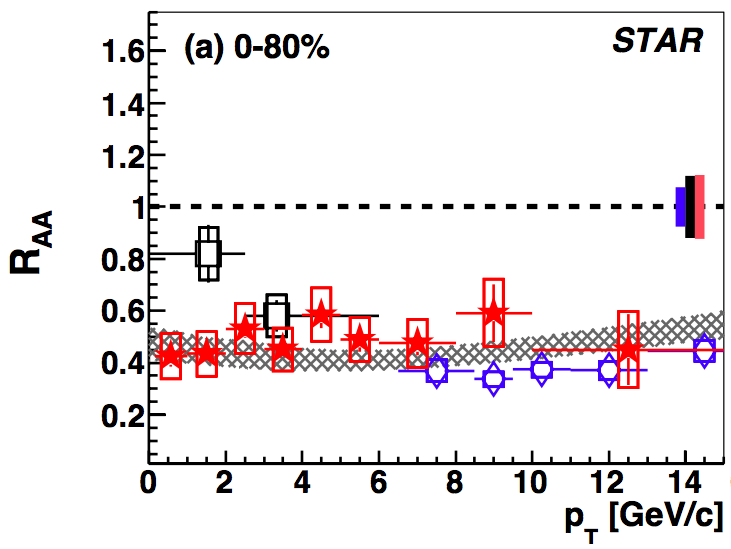
\includegraphics[width=0.47\textwidth]{Figures/Chapter1/STARPt.png}
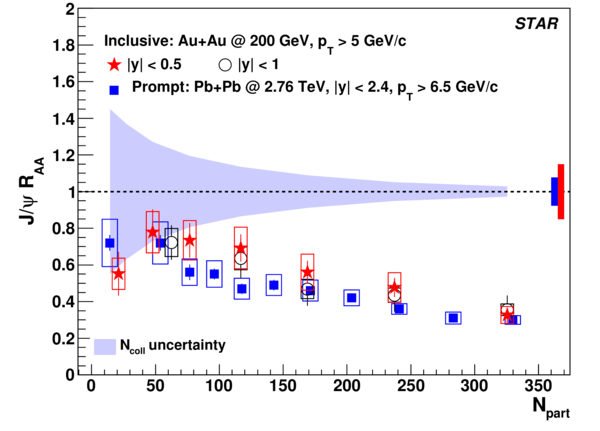
\includegraphics[width=0.487\textwidth]{Figures/Chapter1/STARNPart.png}
\caption{The nuclear modifications factor $R_{AA}$ of fully reconstructed $J/\psi$ as a function of $p_{T}$ (left) and $N_{part}$ (right) measured by the STAR experiment (red data points) at RHIC and CMS (blue diamond data points) and the ALICE (blue circle data points) experiment at the LHC are shown above. We can see that the $J/\psi$ $R_{AA}$ is below 1 for both $p_T$ and $N_{part}$. There is no significant $p_T$ dependence of $J/\psi$ $R_{AA}$. The $J/\psi$ $R_{AA}$ decreases as $N_{part}$ increases, consistent to the increasing creation probability of QGP with larger $N_{part}$.}
\label{JPsiSupp}
\end{center}
\end{figure} 

In fact, we could see that $R_{AA} < 1$ for every data point, which indicates a clear suppression of $J/\psi$ production from experiments at both RHIC and the LHC. However, we should note that the larger $J/\psi$ $R_{AA}$ observed at the LHC compared to RHIC could be explained by regeneration mechanism \cite{JPsiRegen}. The observation of $J/\psi$ suppression is one of the earliest evidence of the discovery of QGP.

Similarly, we expect to see this in $\Upsilon$, which is made of $b \bar b$. Indeed, they expect to have sequential suppression since we have 3 $\Upsilon$ states: $\Upsilon(1S)$,  $\Upsilon(2S)$, and $\Upsilon(3S)$  could be observed in experiments. Because the energy of the $b \bar b$ system or equivalently the rest mass: $m_{\Upsilon(3S)} > m_{\Upsilon(2S)} > m_{\Upsilon(3S)}$, a sequential suppression: $R_{AA}^{\Upsilon(1S)} > R_{AA}^{\Upsilon(2S)} > R_{AA}^{\Upsilon(3S)}$ should be observed if QGP is created. Figure \ref{UpsilonSupp} shows the measurement of fully reconstructed $\Upsilon$ states at RHIC and LHC \cite{STARUpsilonRef,CMSUpsilonRef}

\begin{figure}[hbtp]
\begin{center}
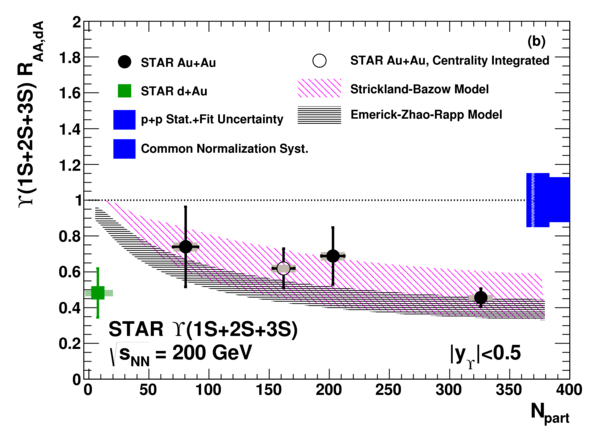
\includegraphics[width=0.52\textwidth]{Figures/Chapter1/STARUpsilon.png}
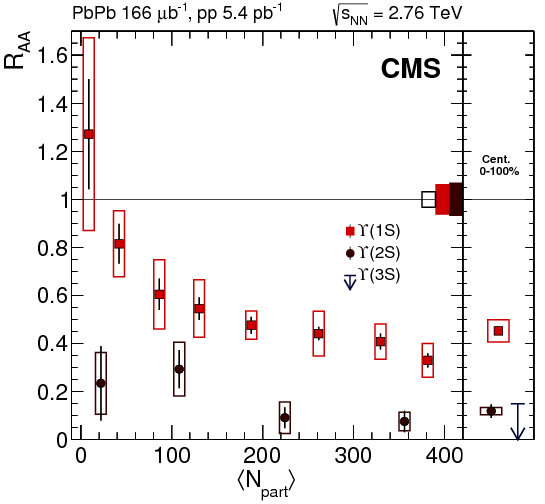
\includegraphics[width=0.40\textwidth]{Figures/Chapter1/CMSUpsilon.png}
\caption{The nuclear modifications factor $R_{AA}$ of fully reconstructed $\Upsilon$ as a function of $N_{part}$ measured by the STAR experiment (left) at RHIC and CMS experiment (right) at the LHC are shown above. We can see that $R_{AA}$  of the three $\Upsilon$ states is below 1 for both $N_{part} > 3$. The $J/\psi$ $R_{AA}$ decreases as $N_{part}$ increases, consistent to the increasing creation probability of QGP with larger $N_{part}$. In addition, a sequential suppression of $\Upsilon$ $R_{AA}$ is observed by the CMS experiment: $R_{AA}^{\Upsilon(1S)} > R_{AA}^{\Upsilon(2S)} > R_{AA}^{\Upsilon(3S)}$, which agrees with the expectation QGP color screening effect.}
\label{UpsilonSupp}
\end{center}
\end{figure} 


\subsection{Jet Quenching} 

Experimentally, due to color confinement, it is impossible to directly detect and track the energetic parton. Therefore, physicists define jet as a spray of collimated hadrons within a narrow cone initiated from the color charged parton. In nuclear and particle physics, jets are used to study the dynamics of partons before hadronization \cite{HERAJET} and understand the properties of QGP \cite{}. A schematic view of a di-jet production from di-qurark event in electron-positron collider $e^+e^-\rightarrow q \bar q$ is shown below in Figure \ref{dijet}


\begin{figure}[hbtp]
\begin{center}
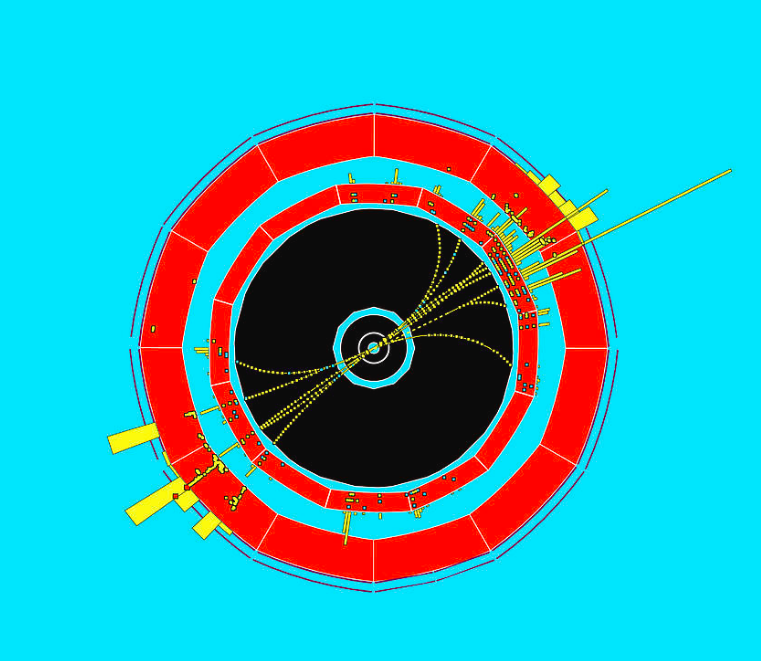
\includegraphics[width=0.50\textwidth]{Figures/Chapter1/DijetEvt.png}
\caption{The schematic display of a di-jet event from the ALEPH (a particle detector at the Large Electron-Positron collider) Experiment at the Large Electron-Positron Collider (LEP) is shown above. We can see two sprays of back to back particles within narrow cone, representing a di-jet event.}
\label{dijet}
\end{center}
\end{figure} 


Since we know QGP a color deconfined phase of matter, an energetic parton carrying color charge traveling through the QGP medium is expected to lose a substantial a mount its energy to the medium. This is similar the effect that an electron beam losing energy in the electron-ion plasma via electromagnetic interaction \cite{}. We call this effect as jet quenching. Figure \ref{JetELoss} shows jet quenching in QGP in AA collisions compared to pp collisions

\begin{figure}[hbtp]
\begin{center}
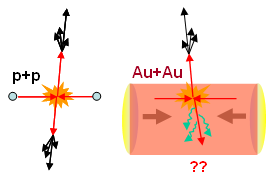
\includegraphics[width=0.45\textwidth]{Figures/Chapter1/JetELoss.png}
\caption{The schematic picture explaining jet quenching is shown above. Hard scatterings in pp collisions produce back-to-back "jets" of particles, but in AuAu collisions, the presence QGP modifies the jets' properties.}
\label{JetELoss}
\end{center}
\end{figure} 


Experimentally, compared to pp collision where QGP is not expected to be created, the jet spectra is modified by the QGP medium. The angular distributions would be broaden due to interaction with the medium and the $p_T$ spectra will be shifted to the left due to energy loss. This can be quantified by jet nuclear modification factor $R_{AA}$ similar to the $R_AA$ for quarkonium suppression mentioned in the previously. Figure \ref{JetRAA} Shows the hadron angular correlation with the STAR experiment at RHIC and jet $R_{AA}$ as a function of $p_T$ with the ALICE experiments at LHC \cite{STARJetRef,ALICEJetRef}:
  
\begin{figure}[hbtp]
\begin{center}
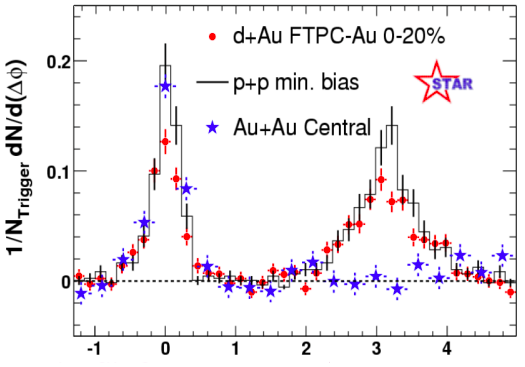
\includegraphics[width=0.55\textwidth]{Figures/Chapter1/HadronAngularSTAR.png}
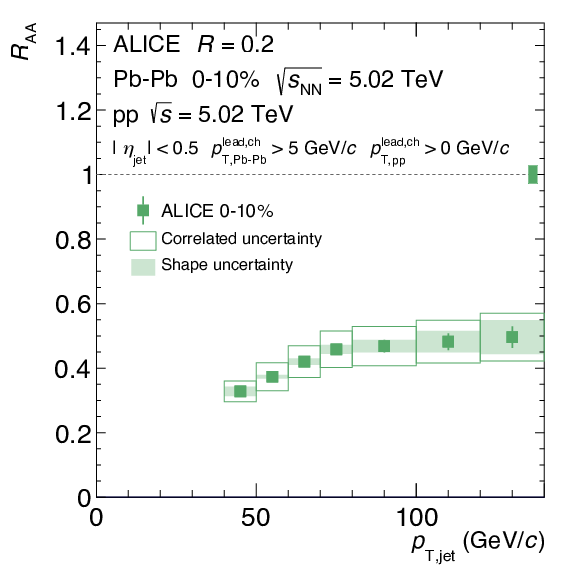
\includegraphics[width=0.40\textwidth]{Figures/Chapter1/JetRAAALICE.png}
\caption{Comparison of two-particle azimuthal distributions for central dAu collisions to those seen in pp and central AuAu collisions measured with the STAR experiment jet $R_{AA}$ as a function $p_T$ measured by the ALICE experiment at LHC (right). From the STAR result, in central AuAu collisions, the back-to-back peak has disappeared due to the transfer of jet energy to the slow expanding medium constituents. The jet $R_{AA}$ from ALICE measurement is clearly below 1, suggesting jet losing a significant fragment of its energy in AA collision compared to pp.}
\label{JetRAA}
\end{center}
\end{figure} 

The jet $R_{AA}$ are all below 1 at RHIC and LHC, which suggest jet quenching in AA collisions, supporting existence of QGP.

\subsection{Elliptic Flow} 

The reaction region in heavy-ion collisions, where the two nuclei overlap with each other, has an almond shape, which is azimuthally asymmetric. If a color deconfined matter QGP is created, particles emitted from the almond shape fire ball are expected to be anisotropic due to differences of the pressure gradient of the QGP in the and their path length through QGP in the x and y direction. Experimentally, physicists Dr. Arthur Poskanzer who sadly just passed away in June 30 2021, and Dr. Sergey Voloshin developed the event plane method to analyze the azimuthal anisotropy of particle emission in heavy-ion collisions \cite{EllipticFlow}. The reaction plane is defined as the plane of the impact parameter and the x-axis. Figure \ref{EventPlane} schematically shows the definition of reaction plane in heavy-ion collisions.

\begin{figure}[hbtp]
\begin{center}
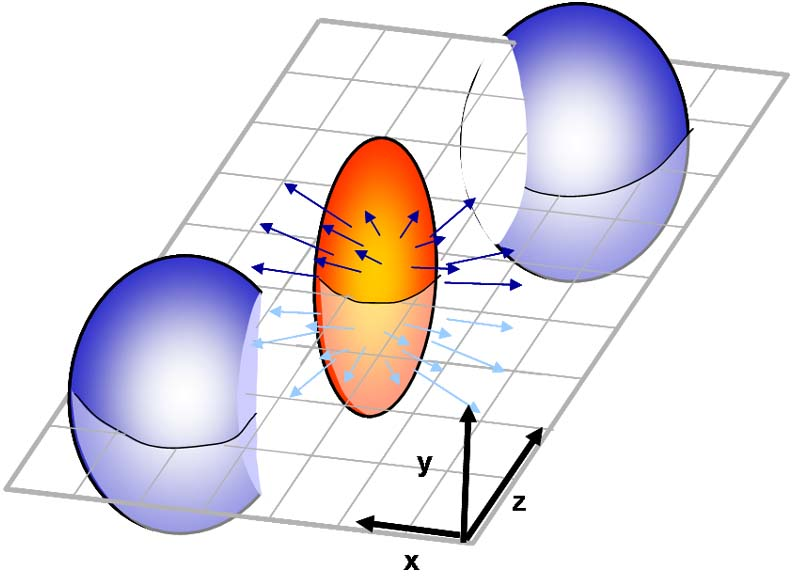
\includegraphics[width=0.40\textwidth]{Figures/Chapter1/ReactionPlane.jpg}
\caption{The figure above shows the ellipsoid of the overlapping nuclear reaction region of two nuclei in heavy-ion collisions. The reaction plane, which is the x-z plane shown as above, is constructed by the beam direction and the impact parameter vector. The emissions of particles are azimuthally anisotropic in the x-y plane.}
\label{EventPlane}
\end{center}
\end{figure} 

The particle spectra in heavy-ion collisions can be factorized as 

\begin{equation}
E \frac{d^3N}{d^3p} = E \frac{1}{2 \pi p_T}\frac{d^3N}{dp_T dy d\phi} = E \frac{1}{2 \pi p_T} \frac{d^2N_1}{dp_T dy} \frac{dN_2}{d\phi}
\end{equation}

Since the particle emission is azimuthally anisotropic, we can expand the $F(p_T,\phi,y) = \frac{dN_2}{d\phi}$ into a Fourier series \cite{EllipticFlow}:


\begin{equation}
F(p_T,\phi,y) = \frac{x_0(p_T,y)}{2\pi}  + \sum_{n=1}^{\infty}[x_n(p_T,y)\cos(n\phi)+y_n(p_T,y)\sin(n\phi)] 
\end{equation}

According to trigonometry, we get

\begin{equation}
F(p_T,\phi,y)  = \frac{x_0(p_T,y)}{2\pi} + \sum_{n=1}^{\infty}2v_n(p_T,y)\cos[n(\phi - \Psi_{n})]
\end{equation}

Here, $v_n = \frac{1}{2} \sqrt{x_n^2 + y_n^2}$ and $\Psi_{n} =\frac{1}{n} \arctan(\frac{y_n}{x_n})$. 

To find the Fourier coefficients $v_n$, we can apply the Fourier tricks to find $x_n$ and $y_n$.


Theoretically, because the function $\frac{dN_2(\phi)}{d\phi}$ is continuously analytical, we can use integral to find the Fourier coefficients [18] 
\begin{equation}
x_n =2\int_{0}^{2\pi} \frac{dN_2(\phi)}{d\phi}\cos(n\phi)d\phi 
\end{equation}
\begin{equation}
y_n =2\int_{0}^{2\pi} \frac{dN_2(\phi)}{d\phi}\sin(n\phi)d\phi 
\end{equation}

Experimentally, because our data take on discrete values, we can convert the integral into a sum 
\begin{equation}
x_n =\frac{2}{N}\sum_{n=1}^{N} \cos(n\phi)d\phi = 2\langle \cos n\phi \rangle
\end{equation}
\begin{equation}
y_n =\frac{2}{N}\sum_{n=1}^{N} \sin(n\phi)d\phi = 2\langle \sin n\phi \rangle
\end{equation}

Here, we sum up all tracks in the experiment to get the $x_n$ and $y_n$. Then, we will be able to find 

\begin{equation}
v_n = \frac{1}{2} \sqrt{x_n^2 + y_n^2} = \sqrt{(\langle \cos n\phi \rangle)^2+(\langle \sin n\phi \rangle)^2}. 
\end{equation}




In heavy-ion physics, the first order Fourier coefficient $v_1$ is called the directed flow. 

\begin{equation}
v_1 =  \sqrt{(\langle \cos \phi \rangle)^2+(\langle \sin \phi \rangle)^2}. 
\end{equation}

It can be connected to the initial tilting source of the colliding nuclei \cite{V1Tilted} and can be used to study Chiral Magnetic Effect \cite{V1CME}. 

The second order Fourier coefficient $v_2$ is called elliptic flow. 

\begin{equation}
v_2 =  \sqrt{(\langle \cos 2\phi \rangle)^2+(\langle \sin 2\phi \rangle)^2} =  \sqrt{(\langle \cos^2 \phi \rangle - \langle \sin^2 \phi \rangle)^2 + (2  \langle \sin \phi \rangle \langle \cos \phi \rangle)^2}. 
\end{equation}

Assuming in initial stage before the collision, the sum of the momentum of two colliding nuclei $\vec p_1$ and $\vec p_2$ is exactly 0 without any fluctuation. That is

\begin{equation}
\vec{p_1} + \vec{p_2} = 0
\end{equation}

According to momentum conservation, for the final state particles, we have 

\begin{equation}
\sum_i^N p_x^i = 0
\end{equation}

\begin{equation}
\sum_i^N p_y^i = 0
\end{equation}

Therefore, we have

\begin{equation}
\langle p_T \cos \phi \rangle = \langle p_x \rangle = \frac{1}{N} \sum_i^N p_x^i   = 0
\end{equation}

\begin{equation}
\langle p_T \sin \phi \rangle = \langle p_y \rangle =  \frac{1}{N} \sum_i^N p_y^i  = 0
\end{equation}
 
But since the $p_T$ and $\phi$ are completely orthogonal, the random variable $p_T$ is uncorrected to $\phi$. Therefore, we have 
 
\begin{equation}
\langle p_T \cos \phi \rangle =  \langle p_T \rangle \langle  \cos \phi \rangle = 0
\end{equation}

\begin{equation}
\langle p_T \sin \phi \rangle =  \langle p_T \rangle \langle  \sin \phi \rangle = 0
\end{equation}

Finally, we know that $p_T > 0$, thus   
 
\begin{equation}
\langle p_T \rangle > 0
\end{equation}  
 
Hence,  


\begin{equation}
\langle \cos \phi \rangle =  0
\end{equation} 


\begin{equation}
\langle \sin \phi \rangle =  0
\end{equation}

Therefore, we have 

\begin{equation}
v_2 = \sqrt{(\langle \cos^2 \phi \rangle - \langle \sin^2 \phi \rangle)^2 + (2  \langle \sin \phi \rangle \langle \cos \phi \rangle)^2} = \langle \cos^2 \phi \rangle - \langle \sin^2 \phi \rangle. 
\end{equation}

In terms of momentum $p_x$ and $p_y$, we can rewrite $v_2$ as 

\begin{equation}
v_2 =  \langle \cos^2 \phi \rangle - \langle \sin^2 \phi \rangle = \langle\frac{p_x^2}{p_T^2} \rangle - \langle \frac{p_y^2}{p_T^2} \rangle = \langle \frac{p_x^2 - p_y^2}{p_T^2} \rangle = \langle \frac{p_x^2 - p_y^2}{p_x^2 + p_y^2} \rangle. 
\end{equation}

Classically, we know that the momentum is proportional to the pressure gradient. Schematically, we could write

\begin{equation}
p_x \simeq \frac{m\tau}{\rho}\frac{\partial P}{\partial x} \simeq \frac{m\tau}{\rho}\frac{P}{L_x}
\end{equation}

Where $m$ is the mass of the particle, $\tau$ is the life time of the QGP, $\rho$ is the density of the QGP, and $L_x$ is the minor axis of the ellipse in the x direction according to the geometry of Figure \ref{EventPlane}.

Likewise, we have the same relation for $p_y$

\begin{equation}
p_y \simeq \frac{m\tau}{\rho}\frac{\partial P}{\partial y} \simeq \frac{m\tau}{\rho}\frac{ P}{L_y}
\end{equation} 

Here,  $L_y$ is the major axis of the ellipse in the y direction according to the geometry of Figure \ref{EventPlane}. Apparently, $L_y > L_x$. 

Hence, we can write $v_2$ as 
\begin{equation}
v_2 =  \langle \frac{p_x^2 - p_y^2}{p_x^2 + p_y^2} \rangle = \frac{\frac{1}{L_x^2} - \frac{1}{L_y^2}}{\frac{1}{L_x^2} + \frac{1}{L_y^2}} =  \frac{L_y^2 - L_x^2}{L_x^2 + L_y^2}  > 0
\end{equation}

In heavy ion collision, we define the eccentricity $\epsilon_s$ of an ellipse is defined as \cite{V2Eccent}

\begin{equation}
\epsilon_s \equiv \frac{L_y^2 - L_x^2}{L_x^2 + L_y^2}
\end{equation}

Hence, we have

\begin{equation}
v_2 \simeq \epsilon_s
\end{equation}

Therefore, we can see that $v_2$ is essentially proportional to the eccentricity simply based on ellipse geometry of reaction region. Historically, $v_2$ has extensively studied experimentally and theoretically. It turns out light hadrons demonstrate collectivity. Their elliptic flow $v_2$ could be calculated using relativistic viscous hydrodynamics, which we will describe in the next section. If QGP is created, we expect $v_2$ of the light flavor hadrons created direction from the QGP to be positive as we derive above. Figure \ref{V2} show the $v_2$ as a function of $p_T$ of charged light flavor hadrons in heavy-ion collisions at mid-rapidity measured by RHIC and LHC experiment \cite{V2STAR,V2ALICE}

\begin{figure}[hbtp]
\begin{center}
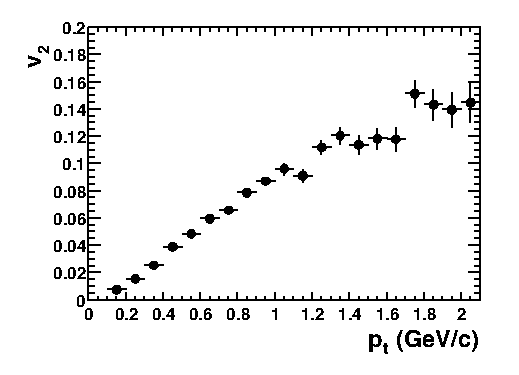
\includegraphics[width=0.45\textwidth]{Figures/Chapter1/STARV2Plot.eps}
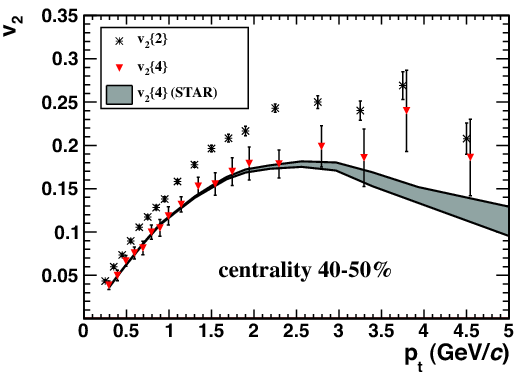
\includegraphics[width=0.45\textwidth]{Figures/Chapter1/ALICEV2Plot.png}
\caption{The elliptic flow of charged particles $v_2$ as a function of $p_T$ in AuAu collision measured by the STAR experiments at RHIC (left) and in PbPb collisions by the ALICE experiments at LHC (right) are shown above. Clearly, $v_2 > 0$ is observed in both experiments.}
\label{V2}
\end{center}
\end{figure}   

We can clearly see positive $v_2$ of charged particles at both RHIC and LHC, which also supports the creation of QGP in high energy heavy-ion collisions.  
 
\subsection{Strangeness Enhancement} 

As described in Section 1.4.6, the temperature of QGP is well above 100 MeV, which is much larger than the strange quark mass (about 95 MeV). Therefore, since $T_{QGP} > m_s$, in thermally and chemically equilibrated QGP, strange quarks could be produced thermally via the pair production process $u \bar u, d \bar d \rightarrow s\bar s$ $gg \rightarrow s \bar s$, creating the chemical abundance equilibrium \cite{SSEnhance}. Therefore, the strangeness content in the QGP is enhanced, which could be experimentally observed from enhancement of strange particle yields in AA collisions compared to pp collisions. A direct experimental observable is the ratio of strange hadron yield to pions in AA and pp collisions. Figure \ref{PhiRAA} shows measurements on strange meson and baryons to pion ratios in AA and pp at RHIC and LHC 

\begin{figure}[hbtp]
\begin{center}
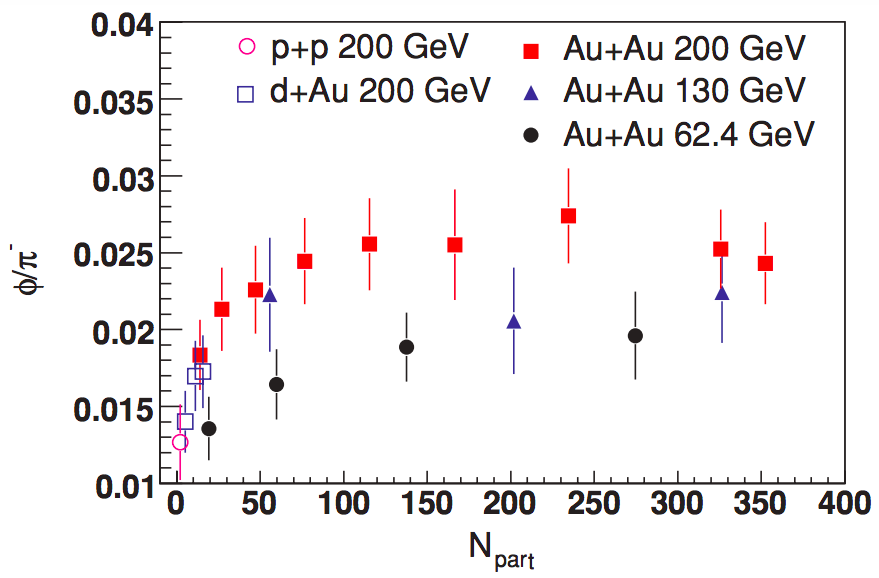
\includegraphics[width=0.45\textwidth]{Figures/Chapter1/STARPhiOverPi.png}
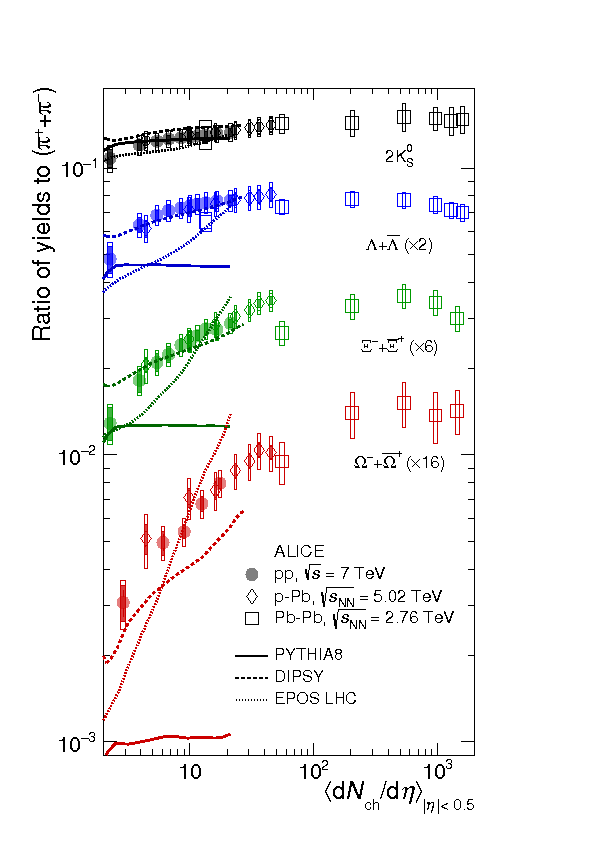
\includegraphics[width=0.30\textwidth]{Figures/Chapter1/ALICEStrange.png}
\caption{The yield ratio of $\phi/\pi$ as a function $N_{part}$ in p + p, p + Au, and Au + Au from the STAR experiment at RHIC (left) and strange hadrons $K^0_s, \Lambda^+, \Xi^0, \Omega^-$ as a function of $\langle dN_{ch}/d\eta \rangle$ from the ALICE experiment at LHC are shown above. We can see a clear trend of the increase of the strange hadron to pion ratio as the event multiplicity increases. In addition, we also see that the $\phi/\pi$ ratio increases as $\sqrt {s_{NN}}$ increases, which suggests the strangeness content enhances as the temperature of the system increase.}
\label{PhiRAA}
\end{center}
\end{figure}   

We can see that $\phi/\pi$ ratio increases as $N_{part}$ and $\sqrt {s_{NN}}$ increases, which indicates strangeness enhancement in AA collisions compare to pp collisions. This again can be served as an evidence for the formation of QGP in heavy-ion collisions at RHIC and LHC. 

%J/psi suppression, jet quenching, elliptic flow, strangeness enhancement 

\subsection{Discovery}

Knowing signatures of QGP, physicists build experiments in heavy-ion colliders to search for QGP. Historically, in a special seminar at CERN February 2000, the discovery of QGP was announce \cite{SPSQGP}. Figure \ref{QGPDisSPS} shows the announcement

\begin{figure}[hbtp]
\begin{center}
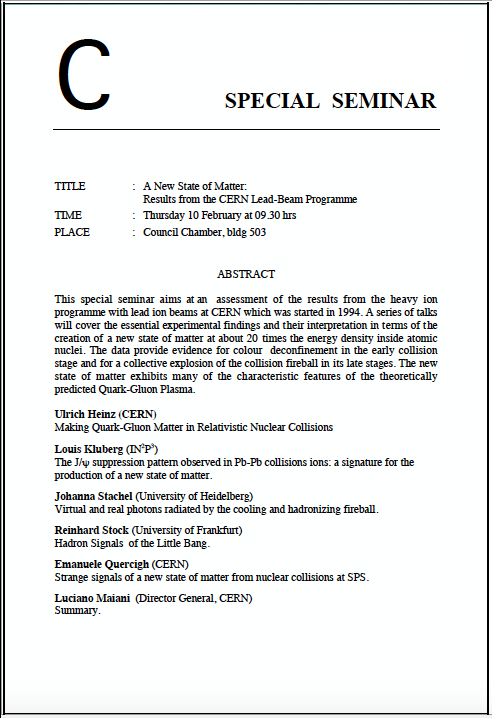
\includegraphics[width=0.90\textwidth]{Figures/Chapter1/QGPDisSPS.png}
\caption{The announcement of discover of QGP in a special seminar at CERN on February 10 2000 is shown above.}
\label{QGPDisSPS}
\end{center}
\end{figure}  

The four typical QGP signatures: quarkonia suppression, jet quenching, elliptic flow, and strangeness enhancement, mentioned previous subsection was also verified by RHIC \cite{BRAHMS,PHOBOS,STAR,PHENIX} and LHC \cite{QGPLHC} later.

\subsection{Macroscopic Properties}

Since the discovery of QGP in laboratories, physicists have conducted extensive studies to pin down its macroscopic properties. 

\textbf{Transient Lifetime:} According to experimental results at RHIC and LHC, QGP has a very short lifetime. It is on the order of 10 fm/c \cite{QGPLifeTime}. It is generally assumed that QGP reaches thermal \cite{QGPThermal} and near chemical equilibrium \cite{QGPChemical} via the strong interaction. So far, there is not sufficient experimental evidence to directly support this assumption.

\textbf{Strong Interacting System:} Moreover, QGP, as a deconfined phase of matter, demonstrates a strongly interacting behavior, which contradicts to the prediction weak coupling according to the asymptotic freedom of quarks and gluons in QCD \cite{QCDAsym}. At $T \sim 1 - 3$ $T_c$, the coupling strength of QGP is still strong: $g_s \sim O(1)$ \cite{sQGP}. Therefore, strong interaction between the QGP constituents is in general non-perturbative. The equation of state of strong interacting QGP, as an input for hydrodynamic calculations, could be reasonably non-pertubative models such as MIT Bag Model or Lattice QCD \cite{LatticeEOS}. 

\textbf{Perfect Liquid Behavior:} Finally, QGP demonstrates a near-perfect liquid properties. The expansion of QGP in the fireball stage is approximately isentropic and could be well described by hydrodynamics \cite{Bjorken}. More specially, due to the relativistic nature of the strongly coupled near-perfect liquid system, assuming QGP reaches thermal \cite{QGPThermal} and near chemical equilibrium \cite{QGPChemical}, relativistic viscous hydrodynamics \cite{4DHydro} is the correct theoretical formalism for the dynamics of QGP. QGP is almost a perfect liquid. Its shear viscosity to entropy density ratio is very small: $\frac{\eta}{s}\sim (1 - 2.5) \frac{1}{4\pi}$ \cite{QGPEtaOverS}, approaching the quantum limit $\frac{\eta}{s} = \frac{1}{4\pi}$ predicted by the strongly coupled N=4 supersymmetric Yang-Mills plasma in Anti-de-Sitter Space/Conform Field Theory (AdS/CFT) correspondence \cite{ADSCFT}.

\textbf{Color Opaque Plasma:} It is also interesting that QGP is a color opaque plasma \cite{QGPGen}. This means that gluons propagating through the QGP will be absorbed by the plasma medium. Experimentally, the suppression of hadrons is a measure of the color opacity of the QGP \cite{QGPGen}. Physicists found that QGP is indeed highly color opaque \cite{QGPOpaque}.


%Nuclear Physics is a study of the interaction of nucleons and structure of atomic nuclei. 
%\subsection{Microscopic Structure}

%Constituents 

%Microscopic Kinetics -- Transport properties
 


\subsection{Open Questions}

Today, it has been more than 20 yeas since the discovery of QGP. However, there are still many outstanding conundrums, most of which are derived from the mysterious macroscopic behavior of QGP. Below is the list of selected open questions and are currently under active investigation by the heavy-ion physics community \cite{BigQuestions}:

1) \textbf{Thermalization of QGP:} How can QGP reach thermal equilibrium within such a short time, which is on the order 1 $fm/c$, from the non-equilibrium stage?

2) \textbf{Inner Workings of QGP:} What is the correct degree of freedom to describe QGP? The inner workings of QGP, as a deconfined phase of matter, must lay between asymptotically free quarks and gluons and color neutral hadrons. That is also why the sPHENIX experiment at RHIC, as the next generation DOE flagship Heavy Ion Physics program in the U.S., is going to built at BNL and collect date to probe the inner workings of QGP by resolving its properties at shorter and shorter length scales. 

3) \textbf{Smallest Droplet of QGP:} What is the smallest droplet of QGP that can be created? Can QGP be created in pPb, pp, or even $e^+e^-$ collision systems? What are the limits of the applicability of hydrodynamics?


\section{Hard Probes}

Traditionally, in Nuclear Physics, when we discover a new state of unknown matter, we use to prepared, clean, known, and controllable probes to scatter of it and look into the scattering patterns of the probes to study its internal structure . Historically, there are many examples. For instance, the Rutherford Scattering using alpha particle to probe the internal structure of atoms \cite{Rutherford} and Deep Inelastic scatter using energetic electrons to probe the internal structure of nucleons \cite{Henry,Richard,Jerry}. Figure \ref{NuclearProbe} shows the schematic picture of Rutherford Scattering and Deep Inelastic Scattering Experiments:

\begin{figure}[hbtp]
\begin{center}
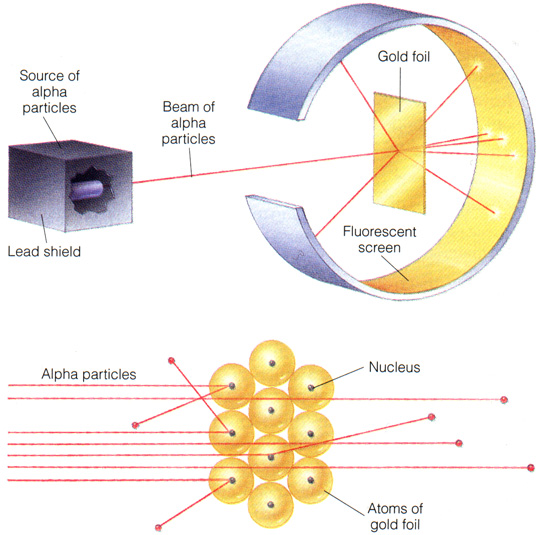
\includegraphics[width=0.45\textwidth]{Figures/Chapter1/Rutherford.jpg}
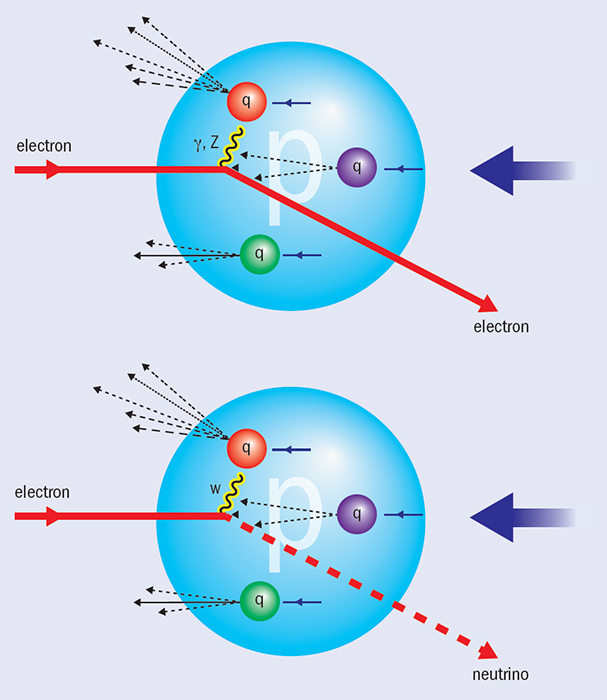
\includegraphics[width=0.45\textwidth]{Figures/Chapter1/DIS.jpg}
\caption{The schematic view of Rutherford scattering (left) and Deep Inelastic Scattering (right) experimental setups are shown above.}
\label{NuclearProbe}
\end{center}
\end{figure}   

Unlike atoms, atomic nuclei, and nucleons, QGP is much more unstable with a transient lifetime. It is in principle impossible to use an external probe to scatter off the QGP and study its microscopic structure. Moreover, since QGP is a color deconfined state of matter, to understand its internal structure, the probe should also be color charged, which is not possible to be prepared externally due to color confinement. Fortunately, in experiments, we could use the other particles produced along with the QGP in heavy-ion collisions and probe the inner workings of the QGP through their interaction with the QGP medium. Particularly, hard probes, such as jets, electroweak bosons, and heavy quarks, are accessible and relativity clean \cite{HardProbes}. In the last two decades, they have been extensively used in the heavy-ion physics community to study QGP \cite{HPSeries}. In the follow subsections, I will briefly introduce the mechanisms of jets, electroweak bosons, and heavy quarks to probe the microscopic structure of QGP in heavy-ion experiments.

\subsection{Jets}

Jet is a relatively hard probe compared to other physics objects. Jets can be used to probe the length scale resolution ability of QGP to resolve the jet internal structure. The study of jet can reveal path length dependence of energy loss $dE/dx$ in the QGP medium. It is essentially a calorimetry of the QCD matter, which is an analog to the energy loss $dE/dx$ of electrically charged particles passing through QED matter used in particle radiation detection \cite{AlphaTheoEx}. From the modification of the jet shape and jet substructure studies in heavy-ion collisions \cite{ModJetSub}, we can understand how jet energy is redistributed to the QGP medium \cite{ALICEJETSub,CMSJetSub}. Experimentally, the observables are di-jet angular correlation, jet $R_{AA}$, and jet fragmentation function. Figure \ref{JetProbe} shows schematically how jets are used to probe the QGP

 \begin{figure}[hbtp]
\begin{center}
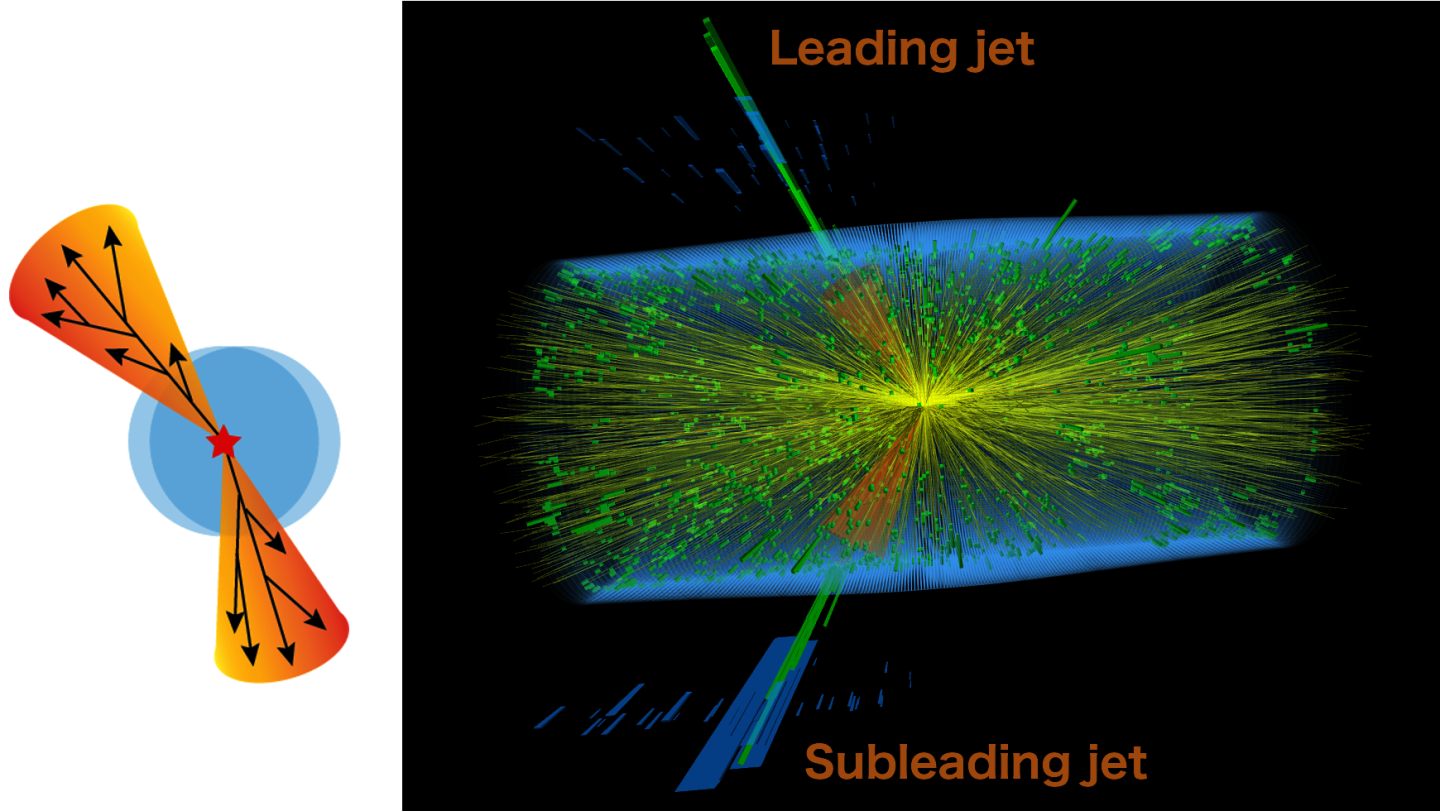
\includegraphics[width=0.60\textwidth]{Figures/Chapter1/CMSJET.png}
\caption{The schematic plot illustrating dijet imbalance (left) compared to the display of original event (right) are shown above. Image from \cite{CMSJETEVENT}.}
\label{JetProbe}
\end{center}
\end{figure}   

\subsection{Electroweak Bosons}

Electroweak bosons, including photon, W, and Z bosons, due to their color neutrality, are relatively clean probes to tag the initial parton dynamics in the QGP. It has shown that they are essentially unmodified as they traverse through the QGP medium. No significant deviation of $R_{AA}$ from unity is observed isolated photon and Z boson measurements in heavy-ion collisions \cite{CMSGammaRef,CMSZRef} as shown in Figure \ref{PhoZV2Ref}

 \begin{figure}[hbtp]
\begin{center}
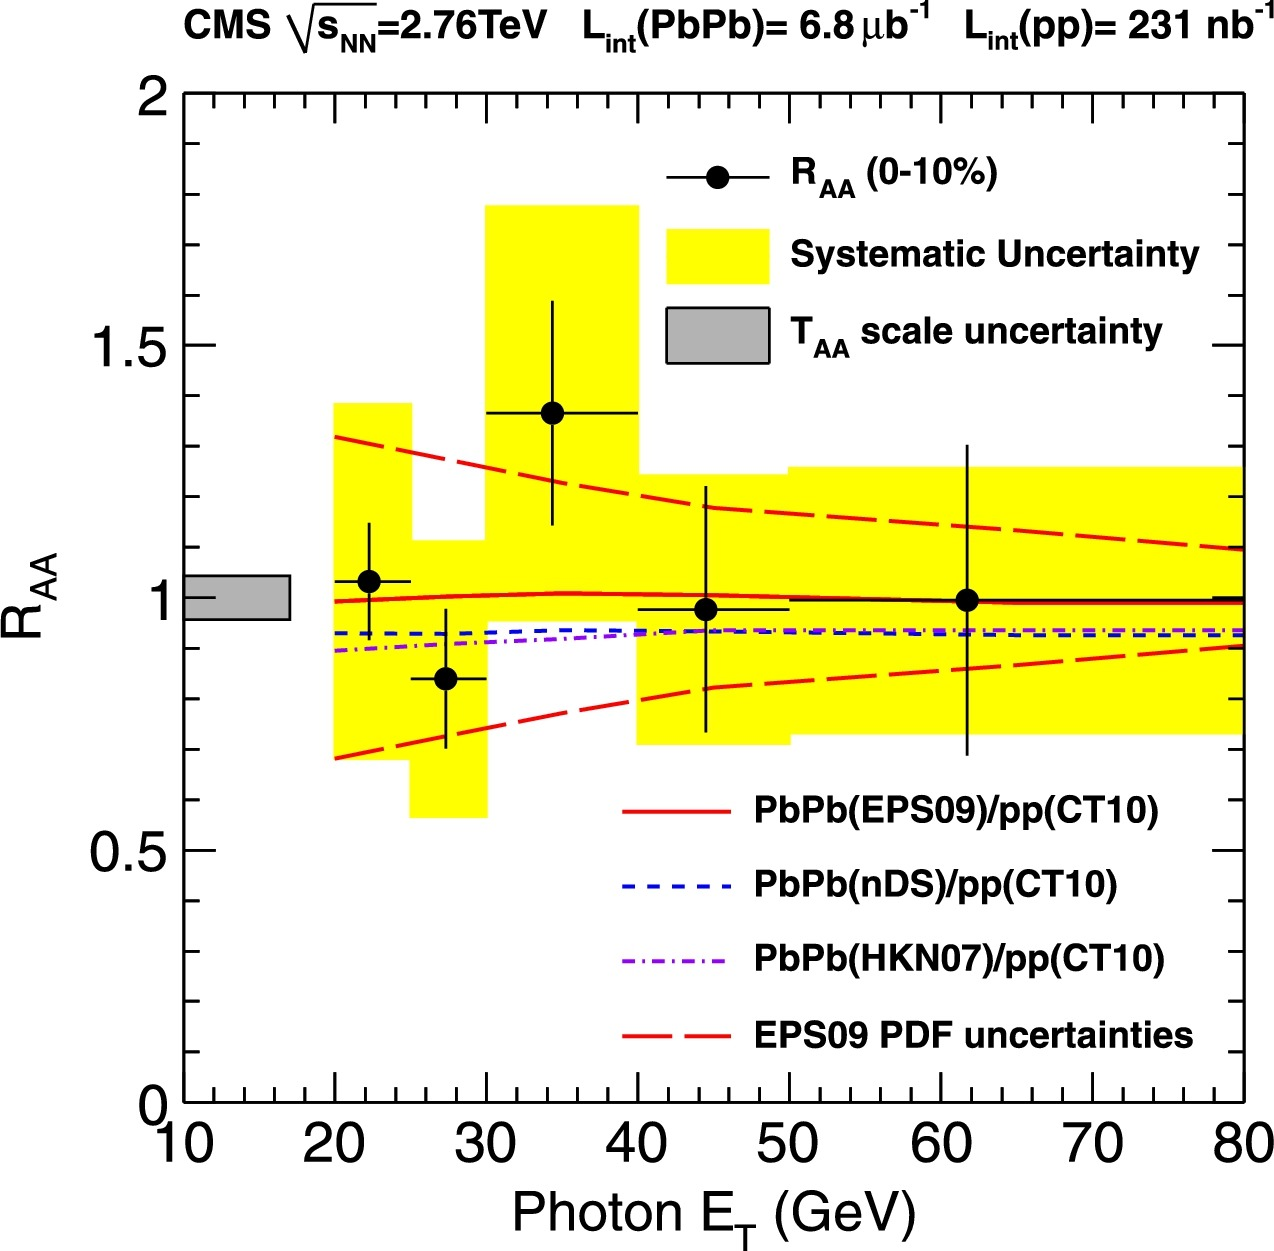
\includegraphics[width=0.45\textwidth]{Figures/Chapter1/GammaRAA.jpg}
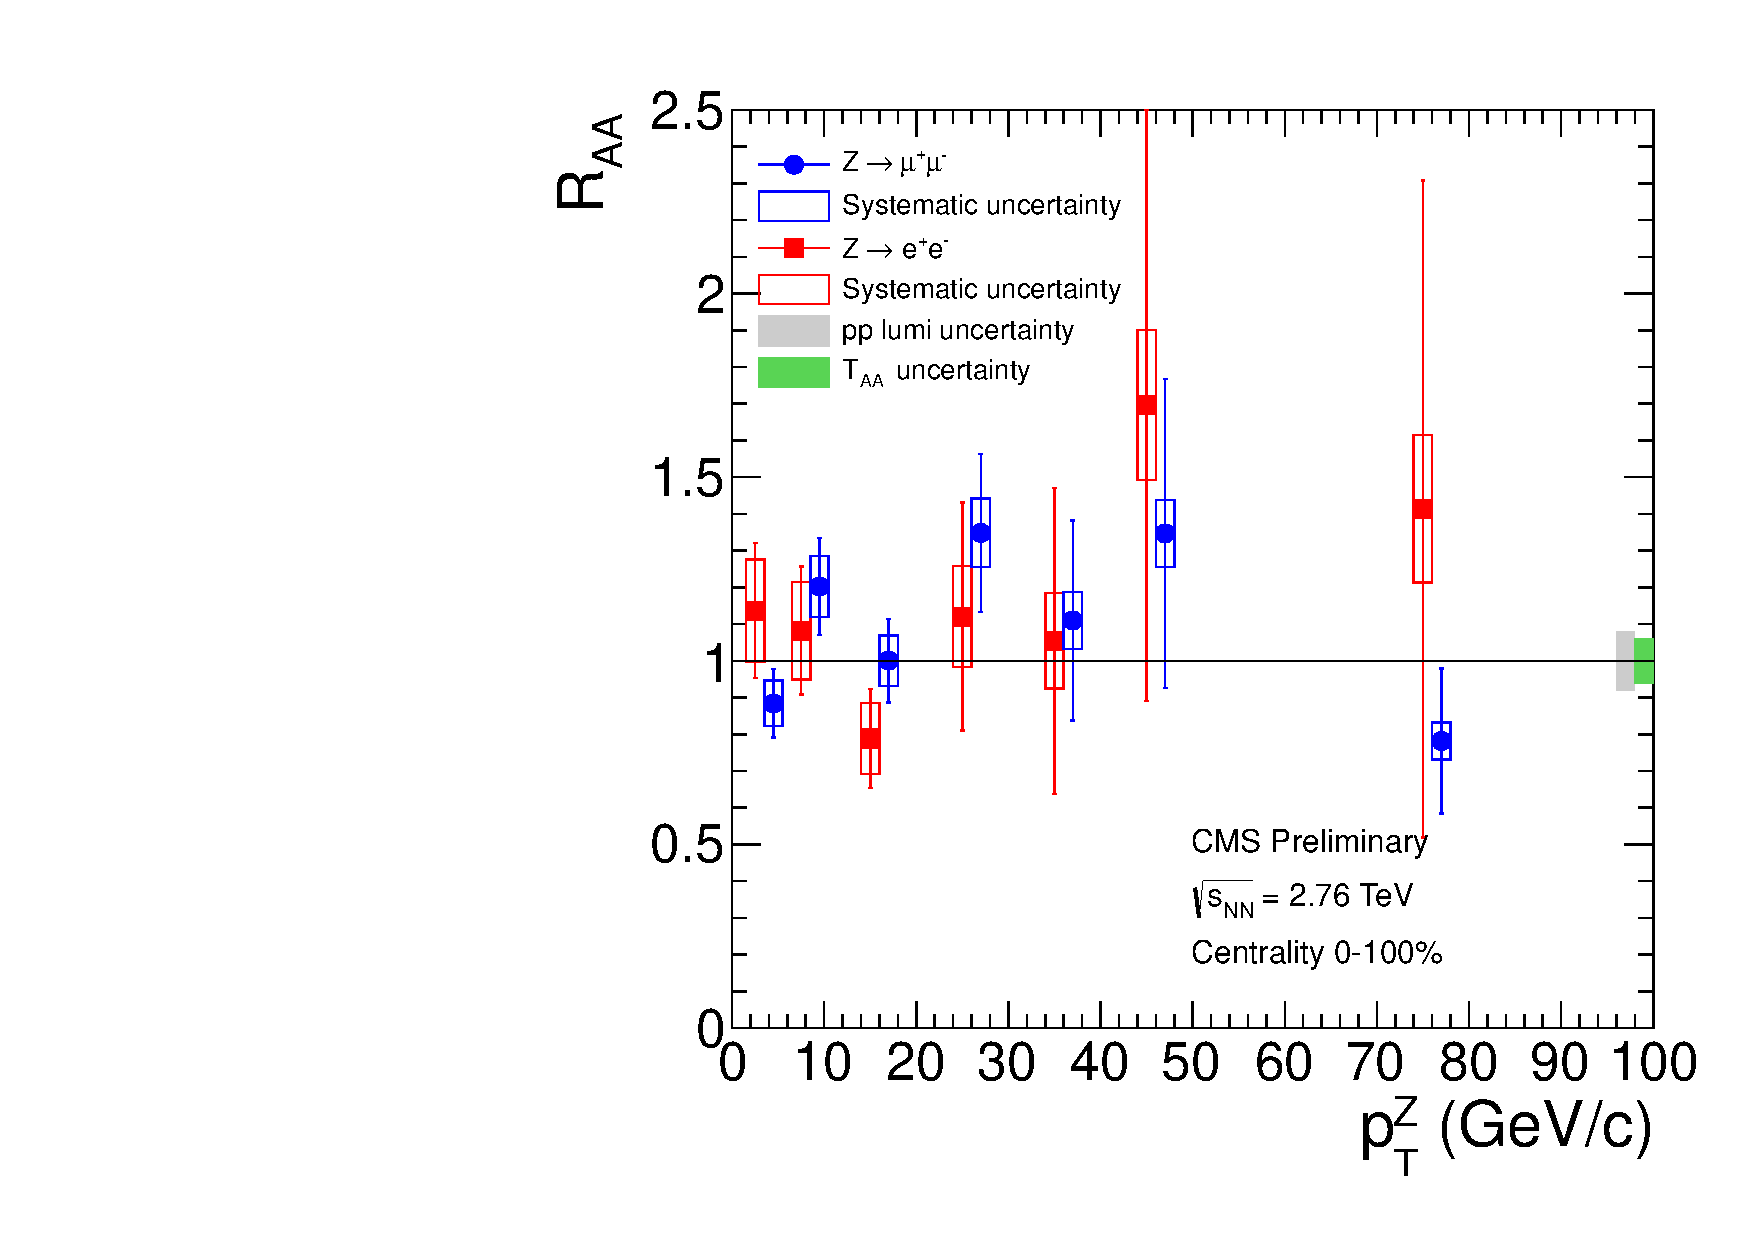
\includegraphics[width=0.45\textwidth]{Figures/Chapter1/ZRAA.pdf}

\caption{The $R_{AA}$ vs $p_T$ of direct photon (left) and Z boson (right) measured with the CMS experiment at LHC are shown above. We could see that the $R_{AA}$ of both photon and Z boson are consistent with unity within their uncertainties.}
\label{PhoZV2Ref}
\end{center}
\end{figure}   

Experimentally, we can study the angular correlation between photon-tagged and Z-tag jets to understand the medium effect to the jet and probe the internal structure of QGP. Figure \ref{BosonTagJet} show schematically an event with a electroweak boson and a jet produced in and propagate through the QGP medium from the Cover in one of the issues of Physical Review Letter \cite{PRLCover}.

 \begin{figure}[hbtp]
\begin{center}
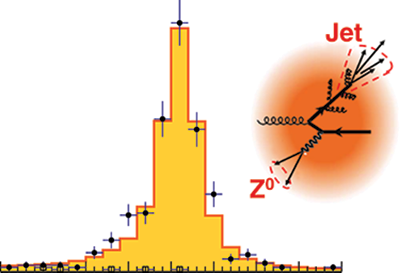
\includegraphics[width=0.45\textwidth]{Figures/Chapter1/ZTagJet.png}
\caption{The schematic plot of a Z + jet event with the creation of QGP and the invariant mass of fully reconstructed Z boson via the decay channel $Z \rightarrow \mu^+ \mu^-$ in the front cover of Physics Review Letter (Volume 119, Issue 8) is shown above. We could see that the Z boson is essentially unmodified by the QGP medium.}
\label{BosonTagJet}
\end{center}
\end{figure}   

\subsection{Heavy Quarks}

Heavy quarks, such as charm and beauty quarks, have large mass compared to the $\Lambda_{QCD}$ and $T_{QGP}$. Therefore, they are predominantly produced in early stage of heavy-ion collisions where hard scattering processes occur. Their production could be calculated by perturbation QCD. Figure \ref{HQProduce} show the lowest order Feynman diagrams of heavy quark pair production in QCD. 

 \begin{figure}[hbtp]
\begin{center}
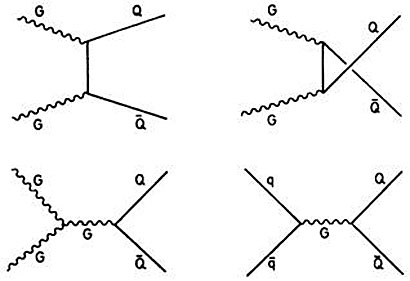
\includegraphics[width=0.45\textwidth]{Figures/Chapter1/HQDiagram.jpg}
\caption{The four lowest order tree level Feynman diagrams of heavy quark pair production are shown above.}
\label{HQProduce}
\end{center}
\end{figure}   

In general, due to their relatively momentum transfer to the medium constituents compared to mass \cite{}, they do not reach complete thermalization via multiple scattering as they traverse through the QGP. In addition, since their lifetime is much longer than the QGP lifetime, they retain their identities and record the evolution of the QGP, which makes them excellent probes. Then, they travel through the medium, hadronize into heavy flavor hadrons, and decay weakly. Their decay product are detected and identified by particles detectors.

Experimentally, from the final stage decay products, we can fully reconstruct open heavy flavor hadrons where heavy quark dynamics is encoded with different transverse momenta to study their diffusion coefficients, hadronizaton mechanism, and energy loss to probe the microscopic structure of QGP via their scattering patterns with the QGP constituents at different wavelengths. Figure \ref{HQ} below shows respectfully an event of beauty heavy quark production and hadronization in vacuum and QGP.

 \begin{figure}[hbtp]
\begin{center}
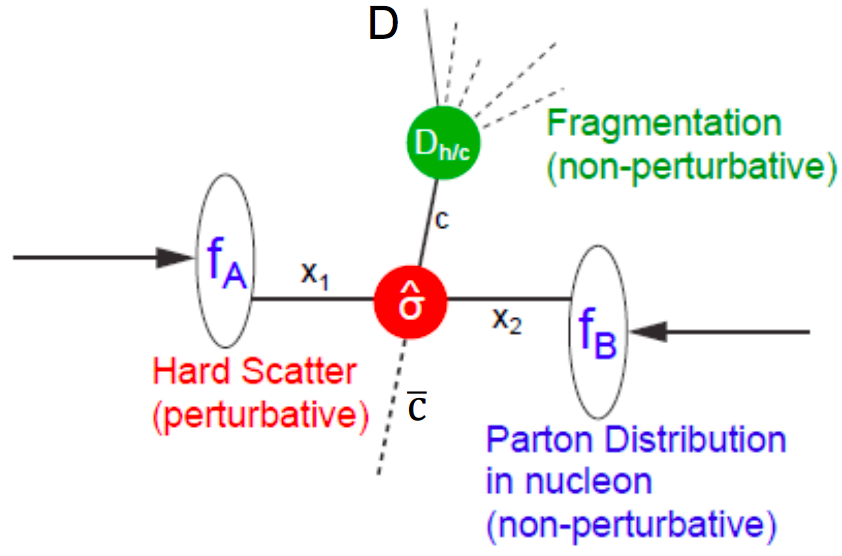
\includegraphics[width=0.46\textwidth]{Figures/Chapter1/HQVacuum.png}
\includegraphics[width=0.48\textwidth]{Figures/Chapter1/HQQGP.png}
\caption{The schematic plots of heavy quark production and hadronization in vacuum (left) and QGP (right) are shown above.}
\label{HQ}
\end{center}
\end{figure}   


\section{Open Heavy Flavor Physics}

My graduate research focuses on answering the second question through the data analysis of fully reconstructed heavy flavor hadrons with the CMS experiment to understand transport properties and probe the microscopic structure of QGP. In this section, we will focus on discussing open heavy flavor physics where the only one heavy quark $Q$ is in hadron. Open heavy flavor hadrons have $\pm 1$ heavy flavor number. Quarkonia states $Q\bar Q$ are considered as hidden heavy flavor with a zero net heavy flavor quantum number. Their properties are different from open heavy flavor hadrons. We will not be discussed them in the follow subsections. 

\subsection{Heavy Quark Physics in Vacuum}

To use heavy quark to probe the QGP created in heavy-ion collisions, we first need to understand heavy quark physics in vacuum from pp collisions. In the process $pp \rightarrow Q \bar Q$, QCD factorization theorem could be applied to study the using perturbative QCD (pQCD). Fixed-to-Next-to-the-Leading (FONLL) is pQCD model calculating the spectra of charm and beauty quarks, schematically denoted as: $\frac{d^2\sigma^Q}{p_T dp_T dy}$, in $pp \rightarrow Q  \bar Q$ at different energies \cite{FONLLRef}. Figure \ref{FONLL} shows the FONLL calculations of charm and beauty quarks spectra produced at the LHC energy for pp collisions at $\sqrt s = 5.02$ TeV.

 \begin{figure}[hbtp]
\begin{center}
\includegraphics[width=0.45\textwidth]{Figures/Chapter1/HQDiagram.jpg}
\caption{The charm quark transverse momentum distribution at $\frac{d\sigma}{dp_T}$ at $|y| < 1$ from FONLL calculations is shown above.}
\label{FONLL}
\end{center}
\end{figure}   

In vacuum, heavy quarks fragment into heavy flavor hadrons $Q \rightarrow H_Q$. We can defined the parton fragmentation function $D^{H_Q}_{i}(z,\mu^2)$ where is the probability for a quark $q$ with energy $E$ fragment into a hadron with energy $zE$ ($0 < z < 1$) at the factorization scale of $\mu^2$ \cite{QCDFFunc}. According to pQCD, $D^{H_Q}_{i}(z,\mu^2)$ is universal in vacuum from $e^+e^-$, $ep$, and $pp$ collisions. Figure \ref{FFProcess} shows the scattering processes which fragmentation fraction is involved:

 \begin{figure}[hbtp]
\begin{center}
\includegraphics[width=1.0\textwidth]{Figures/Chapter1/FFProcess.png}
\caption{Single-inclusive hadron production process, where fragmentation function are involved, in (a) electron-positron annihilation, (b) deep-inelastic lepton-nucleon scattering, (c) proton-proton scattering are shown above.}
\label{FFProcess}
\end{center}
\end{figure}   

Next, we are ready to define heavy quark fragmentation fraction $f(Q \rightarrow H_Q)$. First we know, the energy

\begin{equation}
E=  \sqrt{m^2 + p_T^2 \cosh^2 y}
\end{equation}

Ignoring the mass, we have

\begin{equation}
E \simeq p_T \cosh y
\end{equation}

So energy of hadron $E^h$ that the quark with $E^Q$ fragmented to will be


\begin{equation}
E^h  = z E^Q 
\end{equation}

So we have the transverse momentum of the hadron $p_T^h$ 

\begin{equation}
p_T^{H_Q} = z p_T^Q
\end{equation}

With heavy quark spectra $ \frac{d^2\sigma^Q}{p_T dp_T dy}$ and parton fragmentation function $D_{i}^{H_Q}(z,\mu^2)$, we let


\begin{equation}
 \frac{d^2\sigma^Q}{p_T dp_T dy} = F^Q(p_T, y)
\end{equation}


Hence, for a hadron with $p_T$, the heavy quark will have $p_T/z$ with probability $D^{H_Q}_{i}(z)$ to fragment into this hadron. Therefore, the heavy flavor hadron spectra is given by:

\begin{equation}
\frac{d^2\sigma^{H_Q}}{p_T dp_T dy} = \int_{x_T}^1 F^Q(p_T/z, y) D_{i}^{H_Q}(z,\mu^2) dz
\end{equation}

Here $x_T = \frac{2p_T}{\sqrt s}$ \cite{HadronScale}.







\iffalse



From Figure \ref{FONLL} , it looks like the $p_T$ spectra of heavy quarks is overall approximately power law, particularly at high $p_T$. In fact, at a fixed $x_T$ and the center of mass angle \cite{HadronScale}, the heavy quark spectra overall demonstrates the power like behavior. In addition, assuming the spectra $F^Q(p_T,y)$ factorizes, we have
 

\begin{equation}
F^Q(p_T, y) \sim g(y) p_T^{-n}
\end{equation}

Hence,

\begin{equation}
F^Q(p_T/z, y) \sim F^Q(p_T, y)/z^{-n} = F^Q(p_T, y) z^n
\end{equation}


\begin{equation}
\frac{d^2\sigma^{H_Q}}{p_T dp_Tdy} \simeq \int_{x_T}^1 F^Q(p_T, y)  z^{n} D^{H_Q}_{i}(z) \frac{dz}{z^2} =F^Q(p_T, y)  \int_{x_T}^1  z^{n-2} D^{H_Q}_{i}(z) dz
\end{equation}



Hence, we can define the approximately constant heavy quark fragmentation fraction $f_{Q \rightarrow H_Q}$ as follows

\begin{equation}
f(Q \rightarrow H_Q) = \int_{x_T}^1 z^{n-2} D^{H_Q}_{i}(z) dz
\end{equation}

Hence, we will get 

\begin{equation}
\frac{d^2\sigma^{H_Q}}{p_T dp_T dy} = f(Q \rightarrow H_Q)  \frac{d^2\sigma^Q}{p_T dp_T dy}
\end{equation}

\fi

Now if we consider a factorization scaling near the heavy quark mass $\mu^2 \rightarrow m_Q^2$, according to PDG reference \cite{AlphaTheoEx}, heavy quark fragmentation function $D_Q^{H_Q}(z)$ is in a form of delta function and light quark $q$ and gluons $g$ ($i = g, q$) will not contribute to produce heavy flavor hadrons. Hence, we could right

\begin{equation}
D^{H_Q}_{q,g}(z,\mu^2)|_{\mu^2=m_Q^2} = 0
\end{equation}

\begin{equation}
D^{H_Q}_{Q}(z,\mu^2)|_{\mu^2=m_Q^2} = f(Q \rightarrow H_Q) \delta(1 - z)
\end{equation}

Here $f({Q \rightarrow H_Q})$ is the heavy quark fragmentation fraction and stands for the probability of a heavy quark $Q$ hadronize into an open heavy flavor hadron $H_Q$. Indeed, according to the momentum sum rule constraint of the parton fragmentation function \cite{QCDFFunc}

\begin{equation}
\sum_{H_Q} \int_0^1 z D^{H_Q}_{Q}(z,\mu^2) dz = 1
\end{equation}

\begin{equation}
\sum_{H_Q} \int_0^1 z f(Q \rightarrow H_Q) \delta(1 - z) dz = 1
\end{equation}

\begin{equation}
\sum_{H_Q} f(Q \rightarrow H_Q) = 1 
\end{equation}

This verifies that the sum of heavy quark fragmentation fraction over all heavy flavor hadrons is equal to 1. Next, we have 


\begin{equation}
\frac{d^2\sigma^{H_Q}}{p_T dp_T dy} = \int_{x_T}^1 F^Q(p_T/z, y) D_{i}^{H_Q}(z,\mu^2) dz =  \int_{x_T}^1 F^Q(p_T/z, y) D^{H_Q}_{Q}(z,m_Q^2) dz 
\end{equation}

Thus,

\begin{equation}
\frac{d^2\sigma^{H_Q}}{p_T dp_T dy}  = \int_{x_T}^1 F^Q(p_T/z, y) f(Q \rightarrow H_Q) \delta(1 - z) dz =  f(Q \rightarrow H_Q)  F^Q(p_T, y)
\end{equation}

Hence, we have 

\begin{equation}
\frac{d^2\sigma^{H_Q}}{p_T dp_T dy} = f(Q \rightarrow H_Q) \frac{d^2\sigma^{Q}}{p_T dp_T dy}
\end{equation}

This means that the open heavy flavor hadron spectra $\frac{d^2\sigma^{H_Q}}{p_T dp_T dy}$ is essentially proportional to the heavy quark spectra $\frac{d^2\sigma^{Q}}{p_T dp_T dy}$ with heavy quark fragmentation fraction $f(Q \rightarrow H_Q)$ the as the coefficient of proportionality. Experimentally, charm and beauty fragmentation fractions have been measured at LEP, HERA, and the LHC and documented in PDG \cite{AlphaTheoEx}. The fragmentation fraction is often treated roughly a constant independent to $p_T$, $y$, and $\sqrt s$ and is assumed to be universal in $e^+e^-$, $ep$, and $pp$ collisions systems \cite{AlphaTheoEx}. 

In terms of being a constant, according LHCb $pp$ results \cite{LHCbFF}, it appears that the fragmentation fraction has $p_T$ and $\sqrt s$ dependence while no significant $\eta_B$ (or $y$) dependence is observed. Figure \ref{BeautyFFLHCb} shows the $f_s/(f_d + f_u)$.

 \begin{figure}[hbtp]
\begin{center}
\includegraphics[width=0.33\textwidth]{Figures/Chapter1/LHCbFFs.png}
\caption{Single-inclusive hadron production process, where fragmentation function are involved, in (a) electron-positron annihilation, (b) deep-inelastic lepton-nucleon scattering, (c) proton-proton scattering are shown above.}
\label{BeautyFFLHCb}
\end{center}
\end{figure}   


In terms of universality, according to Strangeness Quark Matter Conference (SQM) in 2021, a hadronization universality breaking is observed from the ALICE experiment at the LHC \cite{GMISQM}. Figure \ref{CharmFFALICE} shows the hadronization universality breaking reported by the ALICE experiment in SQM 2021

 \begin{figure}[hbtp]
\begin{center}
\includegraphics[width=1.0\textwidth]{Figures/Chapter1/FFProcess.png}
\caption{Single-inclusive hadron production process, where fragmentation function are involved, in (a) electron-positron annihilation, (b) deep-inelastic lepton-nucleon scattering, (c) proton-proton scattering are shown above.}
\label{CharmFFALICE}
\end{center}
\end{figure}   

Further investigations of these results are currently ongoing. However, we will not expand the discussions here. Now, equipped with the understanding of heavy flavor physics in vacuum from $pp$ collisions as a reference, we are ready to use heavy quarks to probe the inner workings of QGP created in heavy-ion collisions. 

\subsection{Heavy Quark Diffusion}

In the limit of low $p_T$ or equivalently long wavelength, for heavy quarks inside the QGP medium, their elastic collision cross section dominates. In elastic $Q q \rightarrow Q q$ process in the thermally equilibrated QGP medium, heavy quarks has the relatively small momentum transfers of the order of the temperature compared to the heavy quark mass: $m_Q > |k| \simeq T$. Considering the mean free time of HQ in the QGP medium is about $\tau \sim 0.44 fm/c$ \cite{HQTau}. Therefore, the number of scattering of heavy quarks in the QGP medium is about $n \sim \frac{\tau_{QGP}}{\tau_{HQ}} \simeq 23 \sim O(10)$.

Now, we can consider a simple binomial process to model the diffusion of heavy quark in the QGP medium. Therefore, assuming the momentum of the heavy quark at $t = 0$ is $p$, after the time $\tau_{HQ}$, one scattering happens. The momentum of the heavy quark at $t = \tau_{HQ}$ either $p + k$ or $p - k$. Each has $1/2$ probability. Next, after another $\tau_{HQ}$, another scattering happens. The momentum of the heavy quark at $t = \tau_{HQ}$ either $p + 2k$, $p$ or $p - 2k$ with $1/4$, $1/2$, and $1/2$ probability respectfully. Therefore, the standard deviation of binomial process $\sigma_p = \frac{\sqrt{n}}{2} k$. If we take $n = 25$, $\sigma_p = 2.5k \simeq 2.5 T_{QGP} =$ 0.4 GeV. Experimentally, we consider a heavy quark with momentum about $p  > $ 1GeV/c $> \sigma_p$. 






We could see that the heavy quark transverse momentum is well above 1 GeV/c. Hence, such heavy quarks still retain a lot of memory about its initial conditions after multiple small scattering with QGP medium. Hence, in these conditions, heavy quark undergoes Brownian-like motion in the QGP medium \cite{HQReview}. Their motion in the QGP medium could be characterized by the Planck-Fokker Equation, which could be schematically written as follows \cite{HQRaff}:

\begin{equation}
\frac{\partial}{\partial t} f_q(t, \vec{p}) = \frac{\partial}{\partial p_{i}} \{ A_i(\vec p) f_q(t,\vec{p}) + \frac{\partial}{\partial p_j}[B_{ij}(\vec{p})f_q(t,\vec{p}) ] \}
\end{equation}

Here, $f_q(t,\vec{p})$ is the heavy quark phase space distribution function. If we ignore modification of the cold nuclear matter effect on the heavy quark initial production spectra, then in heavy-ion collision:

\begin{equation}
F^Q( t = 0,p_T) \propto \frac{d\sigma_{FONLL}}{p_Tdp_T}
\end{equation}


The transport parameters $A_i(\vec{p})$ is related to the thermal relaxation rate and $B_{ij}(\vec{p})$ is related to the momentum diffusion of heavy quark \cite{HQReview}. The special diffusion coefficient $D_s$ is related to the transport parameter as follows:

\begin{equation}
D_s = \frac{T} {m_Q A(p=0)}
\end{equation}

$D_s$ characters the fundamental property of the QGP medium via the relationship 

More detailed studies has been carried out to examine heavy quark coupling strength and quantify the information heavy quarks carry as they traverse through the QGP medium \cite{HQJamie}.


\subsection{Heavy Quark Energy Loss}

In the limit of high $p_T$ or equivalently short wavelength, inelastic cross section starts to dominate. Heavy quarks lose a substantial amount of energy as they travel fast through the QGP medium. In a simplified schematization, there are two different pictures that describe the energy loss mechanism of heavy quark in the QGP medium. In the pQCD picture, the coupling of the constituents of the QGP is assumed to be weak. Therefore, the QGP is made of weakly coupled quasiparticles. Heavy quarks scatter off the constituents incoherently when propagating through the QGP medium. There are two energy loss mechanisms: collisional energy loss and radiative energy loss [1]. Figure \ref{} shows schematically heavy quark energy loss mechanism in the QGP medium




The other picture, AdS/CFT, takes the strong coupling limit. In this picture, QGP behave like liquid and heavy quarks scatter off the constituents coherently in the QGP medium. The AdS/CFT model applies holographic drag force [3] to calculate the energy loss of heavy quark [4] in the QGP medium

Dead cone effect, flavor dependence of energy loss. soft gluon radiation dominates


These studies will help us determine  the fundamental jet transport coefficient

\subsection{Heavy Quark Hadronization}

After heavy quarks traverse through the medium, it will hadronize into heavy flavor hadrons, which could be fully reconstructed from their final state decay products. In general, hadronization is non-perturbative \cite{}. Therefore, currently, there is not yet first principle calculation that can describe hadronization.



\subsection{Experimental Observables}

v2

RAA

Ratios

In this thesis, we will focus on the the measurement of experimental observable $B^0_s/B^+$ ratio from fully reconstructed $B^0_s$ and $B^+$ mesons (and their antiparticles) via channels of $B^0_s \rightarrow J/\psi \phi \mu^+ \mu^- K^+ K^-$ and $B^0_s \rightarrow J/\psi K^+ \mu^+ \mu^- K^+$ in pp and PbPb collisions to study the hadronization mechanism of 


